        %%******************************************%%
        %%                                          %%
        %%        Modello di tesi di laurea         %%
        %%            di Andrea Giraldin            %%
        %%                                          %%
        %%             2 novembre 2012              %%
        %%                                          %%
        %%******************************************%%


% I seguenti commenti speciali impostano:
% 1.
% 2. PDFLaTeX come motore di composizione;
% 3. tesi.tex come documento principale;
% 4. il controllo ortografico italiano per l'editor.

% !TEX encoding = UTF-8
% !TEX TS-program = pdflatex
% !TEX root = tesi.tex
% !TEX spellcheck = it-IT

% PDF/A filecontents
\RequirePackage{filecontents}
\begin{filecontents*}{\jobname.xmpdata}
  \Title{Document’s title}
  \Author{Author’s name}
  \Language{it-IT}
  \Subject{The abstract, or short description.}
  \Keywords{keyword1\sep keyword2\sep keyword3}
\end{filecontents*}

\documentclass[10pt,                    % corpo del font principale
               a4paper,                 % carta A4
               twoside,                 % impagina per fronte-retro
               openright,               % inizio capitoli a destra
               english,
               italian,
               "xcolor=table"
               ]{book}

%**************************************************************
% Importazione package
%**************************************************************

\PassOptionsToPackage{dvipsnames}{xcolor} % colori PDF/A

\usepackage{colorprofiles}

\usepackage[a-2b,mathxmp]{pdfx}[2018/12/22]
                                        % configurazione PDF/A
                                        % validare in https://www.pdf-online.com/osa/validate.aspx

%\usepackage{amsmath,amssymb,amsthm}    % matematica

\usepackage[T1]{fontenc}                % codifica dei font:
                                        % NOTA BENE! richiede una distribuzione *completa* di LaTeX

\usepackage[utf8]{inputenc}             % codifica di input; anche [latin1] va bene
                                        % NOTA BENE! va accordata con le preferenze dell'editor

\usepackage[english, italian]{babel}    % per scrivere in italiano e in inglese;
                                        % l'ultima lingua (l'italiano) risulta predefinita

\usepackage{bookmark}                   % segnalibri

\usepackage{caption}                    % didascalie

\usepackage{chngpage,calc}              % centra il frontespizio

\usepackage{csquotes}                   % gestisce automaticamente i caratteri (")

\usepackage{emptypage}                  % pagine vuote senza testatina e piede di pagina

\usepackage{epigraph}			% per epigrafi

\usepackage{eurosym}                    % simbolo dell'euro

%\usepackage{indentfirst}               % rientra il primo paragrafo di ogni sezione

\usepackage{graphicx}                   % immagini

\usepackage{hyperref}                   % collegamenti ipertestuali

\usepackage[binding=5mm]{layaureo}      % margini ottimizzati per l'A4; rilegatura di 5 mm

\usepackage{listings}                   % codici

\usepackage{microtype}                  % microtipografia

\usepackage{mparhack,fixltx2e,relsize}  % finezze tipografiche

\usepackage{nameref}                    % visualizza nome dei riferimenti
\usepackage[font=small]{quoting}        % citazioni

\usepackage{subfig}                     % sottofigure, sottotabelle

\usepackage[italian]{varioref}          % riferimenti completi della pagina

\usepackage{booktabs}                   % tabelle
\usepackage{tabularx}                   % tabelle di larghezza prefissata
\usepackage{longtable}                  % tabelle su più pagine
\usepackage{ltxtable}                   % tabelle su più pagine e adattabili in larghezza
\usepackage{placeins}                   % per \FloatBarrier
\usepackage{mdframed}                   % per contorni immagini
\usepackage[toc, acronym]{glossaries}   % glossario
                                        % per includerlo nel documento bisogna:
                                        % 1. compilare una prima volta tesi.tex;
                                        % 2. eseguire: makeindex -s tesi.ist -t tesi.glg -o tesi.gls tesi.glo
                                        % 3. eseguire: makeindex -s tesi.ist -t tesi.alg -o tesi.acr tesi.acn
                                        % 4. compilare due volte tesi.tex.

\usepackage[backend=biber,style=verbose-ibid,hyperref,backref]{biblatex}
\usepackage{colortbl}
\usepackage{array,booktabs}
\usepackage{float}
\usepackage{listings}
\lstdefinelanguage{GraphQL}{
  keywords = {Query, Mutation, Subscription, union, mutation, subscriptio, query, String, Date, number},
  keywordstyle = \color{DarkOrchid}\bfseries,
  ndkeywords = {type, gigi},
  ndkeywordstyle = \color{BlueViolet}\bfseries,
  comment=[l]{\#},
  morecomment=[s]{/*}{*/},
  commentstyle=\color{Gray}\ttfamily,
  stringstyle=\color{Mahogany}\ttfamily,
  morestring=[b]',
  morestring=[b]"
}
\lstset{
   language=GraphQL,
   extendedchars=true,
   basicstyle=\footnotesize\ttfamily,
   showstringspaces=false,
   showspaces=false,
   numbers=left,
   numberstyle=\footnotesize,
   numbersep=9pt,
   tabsize=2,
   breaklines=true,
   showtabs=false,
   captionpos=b
}
\lstdefinelanguage{JavaScript}{
  %keywords={typeof, new, true, false, catch, function, return, null, catch, switch, var, if, in, while, do, else, case, break},
  %keywordstyle=\color{blue}\bfseries,
  keywords={string, number, Date, typeof, new, true, false, catch, function, return, null, catch, switch, var, if, in, while, do, else, case, break, let},
  keywordstyle=\color{Plum}\bfseries,
  ndkeywords={class, export, boolean, throw, implements, import, this, interface, describe, it},
  ndkeywordstyle=\color{NavyBlue}\bfseries,
  %skewywords={string, numer, Date},
  sensitive=false,
  comment=[l]{//},
  morecomment=[s]{/*}{*/},
  commentstyle=\color{purple}\ttfamily,
  stringstyle=\color{red}\ttfamily,
  morestring=[b]',
  morestring=[b]"
}
\lstset{
   language=JavaScript,
   extendedchars=true,
   basicstyle=\footnotesize\ttfamily,
   showstringspaces=false,
   showspaces=false,
   numbers=left,
   numberstyle=\footnotesize,
   numbersep=9pt,
   tabsize=2,
   breaklines=true,
   showtabs=false,
   captionpos=b
}
                                        % eccellente pacchetto per la bibliografia;
                                        % produce uno stile di citazione autore-anno;
                                        % lo stile "numeric-comp" produce riferimenti numerici
                                        % per includerlo nel documento bisogna:
                                        % 1. compilare una prima volta tesi.tex;
                                        % 2. eseguire: biber tesi
                                        % 3. compilare ancora tesi.tex.

%**************************************************************
% file contenente le impostazioni della tesi
%**************************************************************

%**************************************************************
% Frontespizio
%**************************************************************

% Autore
\newcommand{\myName}{Federico Marchi}
\newcommand{\myTitle}{Analisi comparativa di protocolli di modellazione e trasferimento dati: REST API vs GraphQL}

% Tipo di tesi
\newcommand{\myDegree}{Tesi di laurea}

% Università
\newcommand{\myUni}{Università degli Studi di Padova}

% Facoltà
\newcommand{\myFaculty}{Corso di Laurea in Informatica}

% Dipartimento
\newcommand{\myDepartment}{Dipartimento di Matematica "Tullio Levi-Civita"}

% Titolo del relatore
\newcommand{\profTitle}{Prof.}

% Relatore
\newcommand{\myProf}{Paolo Baldan}

% Luogo
\newcommand{\myLocation}{Padova}

% Anno accademico
\newcommand{\myAA}{2021-2022}

% Data discussione
\newcommand{\myTime}{Dicembre 2022}


%**************************************************************
% Impostazioni di impaginazione
% see: http://wwwcdf.pd.infn.it/AppuntiLinux/a2547.htm
%**************************************************************

\setlength{\parindent}{14pt}   % larghezza rientro della prima riga
\setlength{\parskip}{0pt}   % distanza tra i paragrafi


%**************************************************************
% Impostazioni di biblatex
%**************************************************************
\bibliography{bibliografia} % database di biblatex

\defbibheading{bibliography} {
    \cleardoublepage
    \phantomsection
    \addcontentsline{toc}{chapter}{\bibname}
    \chapter*{\bibname\markboth{\bibname}{\bibname}}
}

\setlength\bibitemsep{1.5\itemsep} % spazio tra entry

\DeclareBibliographyCategory{opere}
\DeclareBibliographyCategory{web}

\addtocategory{opere}{womak:lean-thinking}
\addtocategory{web}{site:agile-manifesto}

\defbibheading{opere}{\section*{Riferimenti bibliografici}}
\defbibheading{web}{\section*{Siti Web consultati}}


%**************************************************************
% Impostazioni di caption
%**************************************************************
\captionsetup{
    tableposition=top,
    figureposition=bottom,
    font=small,
    format=hang,
    labelfont=bf
}

%**************************************************************
% Impostazioni di glossaries
%**************************************************************
\makeglossaries

%**************************************************************
% Acronimi
%**************************************************************
\newacronym[description={\glslink{apig}{Application Program Interface}}]
    {api}{API}{Application Program Interface}

\newacronym[description={\glslink{umlg}{Unified Modeling Language}}]
    {uml}{UML}{Unified Modeling Language}

\newacronym[description={\glslink{ictg}{Information and Communications Tecnology}}]
    {ict}{ICT}{Information and Communications Tecnology}

\newacronym[description={\glslink{ideg}{Integrated Development Environment}}]
    {ide}{IDE}{Integrated Development Environment}
%**************************************************************
% Glossario
%**************************************************************
\newglossaryentry{apig}
{
    name=\glslink{api}{API},
    text=Application Program Interface,
    sort=api,
    description={in informatica con il termine \emph{Application Programming Interface API} (ing. interfaccia di programmazione di un'applicazione) si indica ogni insieme di procedure disponibili al programmatore, di solito raggruppate a formare un set di strumenti specifici per l'espletamento di un determinato compito all'interno di un certo programma. La finalità è ottenere un'astrazione, di solito tra l'hardware e il programmatore o tra software a basso e quello ad alto livello semplificando così il lavoro di programmazione}
}

\newglossaryentry{umlg}
{
    name=\glslink{uml}{UML},
    text=UML,
    sort=uml,
    description={in ingegneria del software \emph{UML, Unified Modeling Language} (ing. linguaggio di modellazione unificato) è un linguaggio di modellazione e specifica basato sul paradigma object-oriented. L'\emph{UML} svolge un'importantissima funzione di ``lingua franca'' nella comunità della progettazione e programmazione a oggetti. Gran parte della letteratura di settore usa tale linguaggio per descrivere soluzioni analitiche e progettuali in modo sintetico e comprensibile a un vasto pubblico}
}

\newglossaryentry{ayce}
{
    name=\glslink{ayce}{All You Can Eat},
    text=All You Can Eat,
    sort=ayce,
    description={con il termine \textit{All You Can Eat} si fa riferimento ai quei ristoranti che permettono di ordinare senza limiti pagando una quota fissa}
}

\newglossaryentry{ideg}
{
    name=\glslink{ide}{IDE},
    text=Integrated Development Environment,
    sort=ide,
    description={in informatica con il termine \textit{Integrated Development Environment} si fa riferimento ad un software che aiuta gli sviluppatori in fase di sviluppo e il debugging del codice di un applicativo.}
}

\newglossaryentry{jv}
{
  name=\glslink{jv}{Java},
  text=Java,
  sort=jv,
  description={in informatica con il termine \textit{Java} si fa riferimento ad un linguaggio di programmazione ad alto livello orientato agli oggetti}
}

\newglossaryentry{ltx}
{
  name=\glslink{jv}{LaTeX},
  text=LaTeX,
  sort=ltx,
  description={con il termine \textit{LaTeX} si fa riferimento ad un linguaggio di marcatura per la preparazione di testi}
}
 % database di termini


%**************************************************************
% Impostazioni di graphicx
%**************************************************************
\graphicspath{{immagini/}} % cartella dove sono riposte le immagini


%**************************************************************
% Impostazioni di hyperref
%**************************************************************
\hypersetup{
    %hyperfootnotes=false,
    %pdfpagelabels,
    %draft,	% = elimina tutti i link (utile per stampe in bianco e nero)
    colorlinks=true,
    linktocpage=true,
    pdfstartpage=1,
    pdfstartview=,
    % decommenta la riga seguente per avere link in nero (per esempio per la stampa in bianco e nero)
    %colorlinks=false, linktocpage=false, pdfborder={0 0 0}, pdfstartpage=1, pdfstartview=FitV,
    breaklinks=true,
    pdfpagemode=UseNone,
    pageanchor=true,
    pdfpagemode=UseOutlines,
    plainpages=false,
    bookmarksnumbered,
    bookmarksopen=true,
    bookmarksopenlevel=1,
    hypertexnames=true,
    pdfhighlight=/O,
    %nesting=true,
    %frenchlinks,
    urlcolor=webbrown,
    linkcolor=RoyalBlue,
    citecolor=webgreen,
    %pagecolor=RoyalBlue,
    %urlcolor=Black, linkcolor=Black, citecolor=Black, %pagecolor=Black,
    pdftitle={\myTitle},
    pdfauthor={\textcopyright\ \myName, \myUni, \myFaculty},
    pdfsubject={},
    pdfkeywords={},
    pdfcreator={pdfLaTeX},
    pdfproducer={LaTeX}
}

%**************************************************************
% Impostazioni di itemize
%**************************************************************
\renewcommand{\labelitemi}{$\ast$}

%\renewcommand{\labelitemi}{$\bullet$}
%\renewcommand{\labelitemii}{$\cdot$}
%\renewcommand{\labelitemiii}{$\diamond$}
%\renewcommand{\labelitemiv}{$\ast$}


%**************************************************************
% Impostazioni di listings
%**************************************************************
\lstset{
    language=[LaTeX]Tex,%C++,
    keywordstyle=\color{RoyalBlue}, %\bfseries,
    basicstyle=\small\ttfamily,
    %identifierstyle=\color{NavyBlue},
    commentstyle=\color{Green}\ttfamily,
    stringstyle=\rmfamily,
    numbers=none, %left,%
    numberstyle=\scriptsize, %\tiny
    stepnumber=5,
    numbersep=8pt,
    showstringspaces=false,
    breaklines=true,
    frameround=ftff,
    frame=single
}


%**************************************************************
% Impostazioni di xcolor
%**************************************************************
\definecolor{webgreen}{rgb}{0,.5,0}
\definecolor{webbrown}{rgb}{.6,0,0}


%**************************************************************
% Altro
%**************************************************************

\newcommand{\omissis}{[\dots\negthinspace]} % produce [...]

% eccezioni all'algoritmo di sillabazione
\hyphenation
{
    ma-cro-istru-zio-ne
    gi-ral-din
}

\newcommand{\sectionname}{sezione}
\addto\captionsitalian{\renewcommand{\figurename}{Figura}
                       \renewcommand{\tablename}{Tabella}}

\newcommand{\glsfirstoccur}{\ap{{[g]}}}

\newcommand{\intro}[1]{\emph{\textsf{#1}}}

%**************************************************************
% Environment per ``rischi''
%**************************************************************
\newcounter{riskcounter}                % define a counter
\setcounter{riskcounter}{0}             % set the counter to some initial value

%%%% Parameters
% #1: Title
\newenvironment{risk}[1]{
    \refstepcounter{riskcounter}        % increment counter
    \par \noindent                      % start new paragraph
    \textbf{\arabic{riskcounter}. #1}   % display the title before the
                                        % content of the environment is displayed
}{
    \par\medskip
}

\newcommand{\riskname}{Rischio}

\newcommand{\riskdescription}[1]{\textbf{\\Descrizione:} #1.}

\newcommand{\risksolution}[1]{\textbf{\\Soluzione:} #1.}

%**************************************************************
% Environment per ``use case''
%**************************************************************
\newcounter{usecasecounter}             % define a counter
\setcounter{usecasecounter}{0}          % set the counter to some initial value

%%%% Parameters
% #1: ID
% #2: Nome
\newenvironment{usecase}[2]{
    \renewcommand{\theusecasecounter}{\usecasename #1}  % this is where the display of
                                                        % the counter is overwritten/modified
    \refstepcounter{usecasecounter}             % increment counter
    \vspace{10pt}
    \par \noindent                              % start new paragraph
    {\large \textbf{\usecasename #1: #2}}       % display the title before the
                                                % content of the environment is displayed
    \medskip
}{
    \medskip
}

\newcommand{\usecasename}{UC}

\newcommand{\usecaseactors}[1]{\textbf{\\Attori Principali:} #1. \vspace{4pt}}
\newcommand{\usecasepre}[1]{\textbf{\\Precondizioni:} #1. \vspace{4pt}}
\newcommand{\usecasedesc}[1]{\textbf{\\Descrizione:} #1. \vspace{4pt}}
\newcommand{\usecasepost}[1]{\textbf{\\Postcondizioni:} #1. \vspace{4pt}}
\newcommand{\usecasealt}[1]{\textbf{\\Scenario Alternativo:} #1. \vspace{4pt}}

%**************************************************************
% Environment per ``namespace description''
%**************************************************************

\newenvironment{namespacedesc}{
    \vspace{10pt}
    \par \noindent                              % start new paragraph
    \begin{description}
}{
    \end{description}
    \medskip
}

\newcommand{\classdesc}[2]{\item[\textbf{#1:}] #2}
                     % file con le impostazioni personali

\definecolor{mygrey1}{HTML}{BCBCBC}
\definecolor{mygrey2}{HTML}{CFCFCF}
\begin{document}
%**************************************************************
% Materiale iniziale
%**************************************************************
\frontmatter
% !TEX encoding = UTF-8
% !TEX TS-program = pdflatex
% !TEX root = ../tesi.tex

%**************************************************************
% Frontespizio 
%**************************************************************
\begin{titlepage}

\begin{center}

\begin{LARGE}
\textbf{\myUni}\\
\end{LARGE}

\vspace{10pt}

\begin{Large}
\textsc{\myDepartment}\\
\end{Large}

\vspace{10pt}

\begin{large}
\textsc{\myFaculty}\\
\end{large}

\vspace{30pt}
\begin{figure}[htbp]
\begin{center}

\includegraphics[height=6cm]{logo-unipd}
\end{center}
\end{figure}
\vspace{30pt} 

\begin{LARGE}
\begin{center}
\textbf{\myTitle}\\
\end{center}
\end{LARGE}

\vspace{10pt} 

\begin{large}
\textsl{\myDegree}\\
\end{large}

\vspace{40pt} 

\begin{large}
\begin{flushleft}
\textit{Relatore}\\ 
\vspace{5pt} 
\profTitle \myProf
\end{flushleft}

\vspace{0pt} 

\begin{flushright}
\textit{Laureando}\\ 
\vspace{5pt} 
\myName
\end{flushright}
\end{large}

\vspace{22pt}

\line(1, 0){338} \\
\begin{normalsize}
\textsc{Anno Accademico \myAA}
\end{normalsize}

\end{center}
\end{titlepage} 
% !TEX encoding = UTF-8
% !TEX TS-program = pdflatex
% !TEX root = ../tesi.tex

%**************************************************************
% Colophon
%**************************************************************
\clearpage
\phantomsection
\thispagestyle{empty}

\hfill

\vfill

\noindent\myName: \textit{\myTitle,}
\myDegree,
\textcopyright\ \myTime.
% !TEX encoding = UTF-8
% !TEX TS-program = pdflatex
% !TEX root = ../tesi.tex

%**************************************************************
% Dedica
%**************************************************************
\cleardoublepage
\phantomsection
\thispagestyle{empty}
\pdfbookmark{Dedica}{Dedica}

\vspace*{3cm}

\begin{center}
De omnibus dubitandum. \\ \medskip
--- Cartesio
\end{center}

\medskip

% !TEX encoding = UTF-8
% !TEX TS-program = pdflatex
% !TEX root = ../tesi.tex

%**************************************************************
% Sommario
%**************************************************************
\cleardoublepage
\phantomsection
\pdfbookmark{Sommario}{Sommario}
\begingroup
\let\clearpage\relax
\let\cleardoublepage\relax
\let\cleardoublepage\relax

\chapter*{Sommario}
Le moderne Web Application adottano un disaccoppiamento stretto tra client e backend.\\\\
Soluzioni architetturali come REST garantiscono di poter realizzare API di utilizzo generale fruibili da svariati client, dai browser sino alle più moderne applicazioni mobili.\\\\
Pur essendo REST lo standard de-facto per la scrittura di Web API, esso presenta alcune debolezze che nuovi strumenti sorti negli utlimi anni cercano di superare.\\\\
GraphQL è certamente una delle più recenti e popolari tecnologie che il mercato dell'Information Technology ci mette a disposizione per la realizzazione di Web API.\\\\
Obbiettivo di questa tesi è quello di realizzare una comparazione tra le tecnologie di data fetching REST e GraphQL individuando i vantaggi nell'adozione di una tecnologia rispetto all'altra; le caratteristiche dei due approcci emergono chiaramente durante lo sviluppo e migrazione di una applicazione da un approccio all'altro.
\endgroup

\vfill

% !TEX encoding = UTF-8
% !TEX TS-program = pdflatex
% !TEX root = ../tesi.tex

%**************************************************************
% Ringraziamenti
%**************************************************************
\cleardoublepage
\phantomsection
\pdfbookmark{Ringraziamenti}{ringraziamenti}

\begin{flushright}{
	\slshape    
	``Life is really simple, but we insist on making it complicated''} \\ 
	\medskip
    --- Confucius
\end{flushright}


\bigskip

\begingroup
\let\clearpage\relax
\let\cleardoublepage\relax
\let\cleardoublepage\relax

\chapter*{Ringraziamenti}

\noindent \textit{Innanzitutto, vorrei esprimere la mia gratitudine al Prof. NomeDelProfessore, relatore della mia tesi, per l'aiuto e il sostegno fornitomi durante la stesura del lavoro.}\\

\noindent \textit{Desidero ringraziare con affetto i miei genitori per il sostegno, il grande aiuto e per essermi stati vicini in ogni momento durante gli anni di studio.}\\

\noindent \textit{Ho desiderio di ringraziare poi i miei amici per tutti i bellissimi anni passati insieme e le mille avventure vissute.}\\
\bigskip

\noindent\textit{\myLocation, \myTime}
\hfill \myName

\endgroup


% !TEX encoding = UTF-8
% !TEX TS-program = pdflatex
% !TEX root = ../tesi.tex

%**************************************************************
% Indici
%**************************************************************
\cleardoublepage
\pdfbookmark{\contentsname}{tableofcontents}
\setcounter{tocdepth}{2}
\tableofcontents
%\markboth{\contentsname}{\contentsname} 
\clearpage

\begingroup 
    \let\clearpage\relax
    \let\cleardoublepage\relax
    \let\cleardoublepage\relax
    %*******************************************************
    % Elenco delle figure
    %*******************************************************    
    \phantomsection
    \pdfbookmark{\listfigurename}{lof}
    \listoffigures

    \vspace*{8ex}

    %*******************************************************
    % Elenco delle tabelle
    %*******************************************************
    \phantomsection
    \pdfbookmark{\listtablename}{lot}
    \listoftables
        
    \vspace*{8ex}
\endgroup

\cleardoublepage

\cleardoublepage

%**************************************************************
% Materiale principale
%**************************************************************
\mainmatter
% !TEX encoding = UTF-8
% !TEX TS-program = pdflatex
% !TEX root = ../tesi.tex

%**************************************************************
\chapter{Introduzione}
\label{introduzione}
%**************************************************************
\intro{Il capitolo seguente introduce l'azienda e illustra la struttura del documento.}\\
%**************************************************************
\section{L'azienda}
\FloatBarrier
\begin{figure}[!h]
\centering

\includegraphics[width=0.4\linewidth]{immagini/synclabLogo.jpeg}
%\caption{Logo Synclab.}
\label{controller-service-repository}
\end{figure}
\FloatBarrier
SyncLab S.r.l è un azienda che si occupa di \gls{ict} ed opera in molteplici settori quali: industriale, sanitario, finanziario, logistico, di telecomunicazioni e infine sanitario.\\\\
Nata a Napoli nel 2002 è al giorno d'oggi divisa in sei sedi operative nelle città di Napoli, Roma, Milano, Como, Verona e infine Padova. Conta più di 300 dipendenti e vanta oltre 150 clienti.

\end{figure}

%**************************************************************
\section{Introduzione al progetto e alla soluzione scelta}
L'idea alla base dello stage è quella di effettuare la migrazione di un applicativo aziendale dal protocollo REST a GraphQL. Lo scopo è quello di analizzare la nuova tecnologia mai affrontata dall'azienda e valutare, attraverso la realizzazione di una analisi di comparazione, quale protocollo potesse soddisfare meglio le esigenze dell'applicativo aziendale.\\ \\
Prima di eseguire la migrazione sull'applicativo aziendale è stato scelto di realizzare un prototipo di gestionale aziendale per familiarizzare con le tecnologie e comprendere quale fosse l'approccio corretto per affrontare la migrazione dell'applicativo aziendale al meglio.\\
Trattandosi di un applicativo composto da backend e frontend, il prototipo è stato realizzato seguendo la medesima architettura al fine di comprenderne il funzionamento e fare pratica. É stato implementato inizialmente con REST API per poi effettuarne la migrazione a GraphQL API.\\ \\
L'applicativo aziendale scelto sul quale è stato realizzato il processo di migrazione si chiama SushiLab. SushiLab, pensato e realizzato da alcuni stagisti nei mesi che precedevano il mio stage, si occupa di gesitre le ordinazioni nei ristoranti di sushi nella formula \gls{ayce}. Dunque dopo aver analizzato l'applicativo e compreso il suo funzionamento ne è stata effettuata la migrazione.\\ \\
Al termine della migrazione, prendendo atto di quanto compreso durante la progettazione, lo sviluppo e la migrazione del prototipo e di SushiLab, è stata effettuata una analisi comparativa su tutti gli aspetti che differenziano i due protocolli per la realizzazione di API.
\section{Descrizione del prodotto ottenuto}
Al termine dello stage è stato realizzato:
\begin{itemize}
  \item \textbf{Prototipo}: composto da backend e frontend è stato realizzato in due versioni:
  \begin{itemize}
    \item \textit{Versione REST}: il prototipo è stato realizzato prima con REST API;
    \item \textit{Versione GraphQL}: a partire dalla versione con REST API è stata effettuata la migrazione e dunque si è ottenuta una versione funzionante con GraphQL API;
  \end{itemize}
  \item \textbf{SushiLab con GraphQL API}: è stato realizzata la migrazione dell'applicativo aziendale dalla sua versione con REST API alla versione funzionante con GraphQL API;
  \item \textbf{Analisi comparativa}: è stato realizzato un documento dettagliato sulla comparazione dei due protocolli REST e GraphQL nel quale si sono approfonditi sia gli aspetti prettamente teorici che quelli più pratici.
\end{itemize}
\newpage
\section{Strumenti e tecnologie utilizzati}
\subsection*{IntelliJ IDEA}
\begin{figure}[ht]
  \begin{minipage}[h]{0.3\linewidth}
    \centering
    
\includegraphics[width=0.9\linewidth]{immagini/IntelliJ.png}
  \end{minipage}
  \begin{minipage}[!h]{0.7\linewidth}
    \textit{IntelliJ IDEA} è un \gls{ide} sviluppato da \textit{JetBrains} che agevola nello sviluppo in \gls{jv}.
    É stato utilizzato nello sviluppo del backend del prototipo e durante la migrazione lato backend sia del prototipo che di SushiLab.
  \end{minipage}
\end{figure}
\subsection*{Visual Studio Code}
\begin{figure}[ht]
  \begin{minipage}[h]{0.3\linewidth}
    \centering
    
\includegraphics[width=0.4\linewidth]{immagini/visualStudioCode.png}
  \end{minipage}
  \begin{minipage}[!h]{0.7\linewidth}
    \textit{Visual Studio Code} è un \gls{ide} sviluppato da \textit{Microsoft} che fornisce molte feature per agevolare lo sviluppo.
    É stato utilizzato nello sviluppo del frontend del prototipo e durante la migrazione lato frontend sia del prototipo che di SushiLab.
  \end{minipage}
\end{figure}
\subsection*{Atom}
\FloatBarrier
\begin{figure}[!h]
  \begin{minipage}[h]{0.3\linewidth}
    \centering
    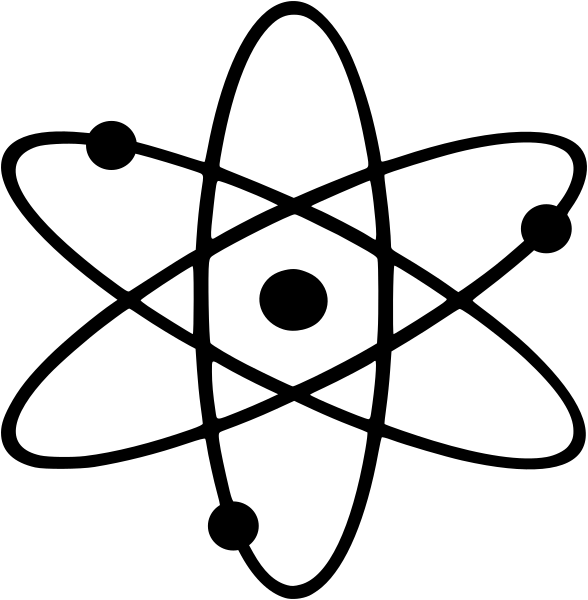
\includegraphics[width=0.5\linewidth]{immagini/atom.png}
  \end{minipage}
  \begin{minipage}[!h]{0.7\linewidth}
    \textit{Atom} è un editor di testo open source. É stato utilizzato durante la stesura con linguaggio \gls{ltx} del documento di analisi comparativa e della documentazione del prototipo e di SushiLab.
  \end{minipage}
\end{figure}
\FloatBarrier
\subsection*{Spring Boot Framework}
\FloatBarrier
\begin{figure}[!h]
  \begin{minipage}[h]{0.3\linewidth}
    \centering
    
\includegraphics[width=0.4\linewidth]{immagini/spring.png}
  \end{minipage}
  \begin{minipage}[!h]{0.7\linewidth}
    \textit{Spring Boot} è un framework open source per lo sviluppo di applicazioni in \gls{jv} strutturate a microservizi. Associati ad esso troviamo molti altri moduli e librerie ampiamente utilizzate nel corso dello stage poiché se integrati permettono di agevolare lo sviluppo. Utilizzato per lo sviluppo e migrazione del prototipo e di SushiLab.
  \end{minipage}
\end{figure}
\FloatBarrier
\subsection*{Angular Framework}
\FloatBarrier
\begin{figure}[!h]
  \begin{minipage}[h]{0.3\linewidth}
    \centering
    
\includegraphics[width=0.5\linewidth]{immagini/angular.png}
  \end{minipage}
  \begin{minipage}[!h]{0.7\linewidth}
    \textit{Angular} è un framework open source per lo sviluppo di applicazioni web. Permette di realizzare Single Page Application che si adattano facilmente a diversi dispositivi. Utilizzato per lo sviluppo e la migrazione del frontend nel prototipo e in SushiLab.
  \end{minipage}
\end{figure}
\FloatBarrier
\subsection*{GitHub}
\begin{figure}[ht]
  \begin{minipage}[h]{0.3\linewidth}
    \centering
    
\includegraphics[width=0.5\linewidth]{immagini/github.png}
  \end{minipage}
  \begin{minipage}[!h]{0.7\linewidth}
    \textit{GitHub} è un servizio di hosting per progetti software. É stato utilizzato per effettuare i salvataggi su cloud del codice e della documentazione sia per quanto riguarda il prototipo che per SushiLab. Permette di tener traccia di tutte le versioni gestite con lo strumento di versionamento Git.
  \end{minipage}
\end{figure}
\subsection*{JUnit 5}
\FloatBarrier
\begin{figure}[!h]
  \begin{minipage}[h]{0.3\linewidth}
    \centering
    
\includegraphics[width=0.6\linewidth]{immagini/JUnit.png}
  \end{minipage}
  \begin{minipage}[!h]{0.7\linewidth}
    \textit{JUnit 5} è un framework di unit testing per il linguaggio di programmazione \gls{jv}. É stato ampiamente utilizzato per effettuare i test di unità nel backend sia del prototipo che dell'applicativo SushiLab.
  \end{minipage}
\end{figure}
\FloatBarrier
\subsection*{Jasmine}
\FloatBarrier
\begin{figure}[!h]
  \begin{minipage}[h]{0.3\linewidth}
    \centering
    
\includegraphics[width=0.4\linewidth]{immagini/jasmine.png}
  \end{minipage}
  \begin{minipage}[!h]{0.7\linewidth}
    \textit{Jasmine} è un framework di test open source. É stato utilizzato in Angular per effettuare i test nel frontend sia del prototipo che dell'applicativo SushiLab.
  \end{minipage}
\end{figure}
\FloatBarrier
\subsection*{Trello}
\FloatBarrier
\begin{figure}[!h]
  \begin{minipage}[h]{0.3\linewidth}
    \centering
    
\includegraphics[width=0.35\linewidth]{immagini/trello.png}
  \end{minipage}
  \begin{minipage}[!h]{0.7\linewidth}
    \textit{Trello} è un software gestionale. É stato utilizzato per tenere traccia di tutti gli sviluppi dello stage nel corso delle varie settimane.
  \end{minipage}
\end{figure}
\FloatBarrier
\subsection*{Discord}
\FloatBarrier
\begin{figure}[!h]
  \begin{minipage}[h]{0.3\linewidth}
    \centering
    
\includegraphics[width=0.7\linewidth]{immagini/discord.png}
  \end{minipage}
  \begin{minipage}[!h]{0.7\linewidth}
    \textit{Discord} è una piattaforma di messaggistica e distribuzione digitale per la comunicazione. É stata utilizzata per la comunicazione con il tutor aziendale e gli altri stagisti.
  \end{minipage}
\end{figure}
\FloatBarrier
%**************************************************************
\newpage
\section{Organizzazione del testo}
\begin{description}
    \item Il {\hyperref[descrizione-stage]{secondo capitolo}} descrive l'analisi preventiva dei rischi, obbiettivi e infine la pianificazione del lavoro;

    \item Il {\hyperref[protocolli-trasmissione-dati]{terzo capitolo}} introduce ai protocolli di modellazione e trasferimento, tra questi approfondisce REST e GraphQL;

    \item Il {\hyperref[casi-uso]{quarto capitolo}} illustra la realizzazione del prototipo con relativa migrazione e la migrazione dell'applicativo SushiLab;

    \item Il {\hyperref[analisi-comparativa]{quinto capitolo}} descrive dettagliatamente l'analisi comparativa tra i protocolli REST e GraphQL;

    \item Il {\hyperref[conclusioni]{sesto capitolo}} riporta le conclusioni finali riguardo lo stage effettuato.
\end{description}
             % Introduzione
% !TEX encoding = UTF-8
% !TEX TS-program = pdflatex
% !TEX root = ../tesi.tex

%**************************************************************
\chapter{Descrizione dello stage}
\label{descrizione-stage}
%**************************************************************

\intro{Breve introduzione al capitolo}\\

%**************************************************************
\section{Introduzione al progetto}

%**************************************************************
\section{Analisi preventiva dei rischi}

Durante la fase di analisi iniziale sono stati individuati alcuni possibili rischi a cui si potrà andare incontro.
Si è quindi proceduto a elaborare delle possibili soluzioni per far fronte a tali rischi.\\

\begin{risk}{Performance del simulatore hardware}
    \riskdescription{le performance del simulatore hardware e la comunicazione con questo potrebbero risultare lenti o non abbastanza buoni da causare il fallimento dei test}
    \risksolution{coinvolgimento del responsabile a capo del progetto relativo il simulatore hardware}
    \label{risk:hardware-simulator}
\end{risk}

%**************************************************************
\section{Requisiti e obiettivi}


%**************************************************************
\section{Pianificazione}
             % Processi
% !TEX encoding = UTF-8
% !TEX TS-program = pdflatex
% !TEX root = ../tesi.tex

%**************************************************************
\chapter{Protocolli di modellazione e trasferimento dati}
\label{cap:protocolli-trasmissione-dati}
%**************************************************************

\intro{Nel seguento capitolo vengono trattati dal punto di vista teorico i protocolli di modellazione e trasferimento dati, in particolare viene approfondito lo stile architetturale REST e il linguaggio di query GraphQL.
}\\

%**************************************************************
\section{Introduzione ai protocolli}
\subsection*{Modello architetturale client-server}
\label{client-server}
Prima di procedere nella spiegazione sui protocolli di trasferimento e modellazione dati, è necessario fare una breve introduzione sull'architettura delle Web Application moderne. Queste seguono ormai tutte un modello server - client, ovvero un modello architetturale che divide in due processi l'applicazione: un client che richiede servizi al server, il quale li esegue ritornando una risposta contenente l'esito dell'operazione. I protocolli di trasferimento e modellazione dati trovano il loro maggior utilizzo proprio nella comunicazione client - server, tuttavia prima di procedere con la loro spiegazione è necessario introdurre il concetto di Application Programming Interfaces.
\subsection*{Application Programming Interfaces}
 Comunemente dette API, ovvero l'acronimo di Application Programming Interfaces, sono interfacce comunemente realizzate per aggevolare la comunicazione tra  server e client. Ciascun applicativo/dispositivo è sviluppato con strutture di dati differenti che evolvono nel tempo, dunque risulta complessa la comunicazione tra queste entità. Le API giocano un ruolo fondamentale nello scambio di dati: infatti definiscono una interfaccia per la comunicazione, la quale è indipendente dall'implementazione specifica del dispositivo o dell'applicativo e permette di comunicare secondo delle regole specifiche riportate nella propria documentazione. Risultano dunque fondamentali nella comunicazione, collaborazione e integrazione di nuovi componenti applicativi.\\ \\
 Al giorno d'oggi le API vengono utilizzate dalla maggior parte delle web applications, dispositivi IoT, applicativi di vario genere e molto altro ancora.
 Nello specifico nella tesi si fa riferimento alle Web API, ovvero a quelle interfacce che sfruttano il protocollo HTTP per la comunicazione con altri applicativi/dispositivi. Ci sono diversi tipi di Web API, tra queste:
 \begin{itemize}
   \item \textbf{API pubbliche}: si tratta di API accessibili da tutti (possono essere anche a pagamento);
   \item \textbf{API private}: si tratta di API create con lo scopo di essere utilizzate solo ed esclusivamente all'interno dell'azienda;
   \item \textbf{API partner}: si tratta di API utilizzate tra aziende in collaborazione;
   \item \textbf{API composte}: si tratta di API differenti combinate tra loro per creare una sequenza di operazioni.
 \end{itemize}
La necessità di standardizzare il modo in cui vengono sviluppate le interfacce API ha portato dunque alla nascita dei protocolli sul trasporto di dati.
\subsection*{Protocolli di trasferimento dati}
Per protocolli di modellazione e trasferimento dati s'intende un insieme di regole, strutture e vincoli che regolano il funzionamento delle API. Permettono dunque di definire una sorta di standard al quale gli sviluppatori possono far riferimento per implementare e interagire con le API. Il termine protocollo non si addice perfettamente a tutte le varie tecnologie di data fetching, tuttavia a grandi linee può racchiuderle e dunque verrà utilizzato per questione di comodità.
\subsection*{I primi protocolli e loro evoluzione}
Al giorno d'oggi il protocollo di modellazione e trasferimento dati più utilizzato è sicuramente REST, tuttavia sono presenti anche altre tipologie di protocolli in utilizzo o che comunque sono state utilizzate in passato. Si tratta di tecnologie con lo stesso scopo, ma di natura completamente differente, di seguito le principali.
\subsubsection*{Remote Procedure Call}
Viene spesso indicato con l'acronimo RPC, si tratta di protocollo secondo il quale una procedura o subroutine viene invocata da un client esterno al server che deve eseguire la procedura, senza che il client conosca i dettagli del network. Viene utilizzato per chiamare processi in sistemi remoti, ma come fossero locali. \\
Di seguito riportata la definizione attribuita all'RPC dagli informatici Andrew Birrell e Bruce Nelson nel 1984:
  \begin{quoting}
    “Meccanismo sincrono che trasferisce il flusso di controllo e i dati attraverso una chiamata di procedura tra due spazi di indirizzo su una rete a banda stretta.”
  \end{quoting}
Come nelle chiamate a procedure locali, un RPC è una operazione sincrona che tiene in pausa il client fino al momento in cui ritorna il risultato della procedura invocata.
\subsubsection*{Simple Object Access Protocol}
Indicato spesso con l'acronimo SOAP, si tratta di un vero e proprio protocollo che definisce la struttura dei dati che devono essere trasferiti e come questi devono essere elaborati. Richiede esclusivamente il formato XML per trasferire dati e tipicamente viene utilizzato il protocollo HTTP per il trasferimento di file, tuttavia possono essere utilizzati anche protocolli differenti come ad esempio il protocollo SMTP. La struttura di un messaggio SOAP è composta da 3 principali componenti:
\begin{itemize}
  \item \textbf{Envelope}: necessario al fine di identificare il documento come messaggio SOAP;
  \item \textbf{Header}: è opzionale. Lo scopo dell'header nei messaggi SOAP è quello di trasportare indicazioni estranee al messaggio che si vuole trasportare, ma che vengono interpretate da i diversi nodi durante il cammino del messaggio;
  \item \textbf{Body}: il body contiene il vero e proprio messaggio che si vuole trasferire.
\end{itemize}
\subsubsection*{Ad hoc}
\section{Approfondimento sullo stile architetturale REST}
REST è l'acronimo di "Representational State Transfer" e si tratta di un tipo di stile architetturale introdotto da Roy Fielding nel 2000 e viene considerato al giorno d'oggi come uno standard per la realizzazione di web API. Si tratta di una astrazione degli elementi di un architettura di un sistema, del quale REST ne ignora i dettagli del'implementazione delle componenti e della sintassi del protocollo imponendo dei vincoli sul loro ruolo e sulla loro interazione.
\subsection*{Principi di un architettura REST}
Un architettura REST dunque deve rispettare alcuni principi, di seguito verranno elencati i sei gruppi definiti da Fielding.
\subsubsection*{Client-server}
Il primo principio sposa uno dei paradigmi cardine dell'informatica, ovvero il principio di \textit{Separation of concerns}, secondo il quale conviene sempre separare un sistema complesso in moduli distinti in modo che ognuno possa avere un proprio compito.\\
Ciò viene ripreso nell'architettura REST separando il client dal server, dunque dividendo due logiche diverse in due moduli distinti. Così facendo server e client possono essere implementati in maniera indipendente, usando qualsiasi lingua o tecnologia, basta che siano conformi al prossimo principio detto \textit{uniform interface}.
\subsubsection*{Uniform interface}
Si tratta di un principio fondamentale che differenzia le REST API da qualsiasi API non REST. Secondo questo prinpicio l'interazione tra componenti Web, dunque client, server e tutti gli intermediari del network, dipendono dalla uniformità delle loro interfacce.\\
I componenti Web dunque sono in grado di comunicare coerentemente seguendo quattro vincoli sull'interfaccia delineati da Fielding; questi sono:
\begin{itemize}
  \item \textbf{Identification of resources}: le risorse che vengono richieste devono essere identificate nella richiesta stessa, dunque specificandole nell'url;
  \item \textbf{Manipulation of resources through representations}: il client deve avere la rappresentazione delle risorse e deve poter sapere come modellarle sul server. L'idea alla base è che la rappresentazione (attraverso un qualsiasi formato, ad es. JSON, XML, ecc...) è una modo per interagire con le risorse, ma non è la risorsa stessa;
  \item \textbf{Self-descriptive messages}: in ciascun messaggio devono esser presenti le informazioni necessarie a descrivere come deve essere processata la richiesta;
  \item \textbf{Hypermedia as the Engine of Application State}: la rappresentazione dello stato di una risorsa deve includere i riferimenti alle risorse correlate. É dunque necessario includere i link per ciascuna risposta, così che il client possa navigare tra le altre risorse facilmente.
\end{itemize}
\subsubsection*{Layered System}
Secondo questo principio l'architettura di un applicativo deve essere composta da più strati. Ciascuno strato inoltre è cieco rispetto agli altri strati, tranne per quanto riguarda gli strati adiacenti. Questi layer possono essere composti da intermediari basati sul network i quali intercettano la comunicazione client-server con uno scopo specifico (ad esempio per questioni di sicurezza, caching, controllo del flusso dati, ecc...), possono essere ad esempio proxy e gateways. Per il principio di Layered System questi intermediari devono aderire alle interfacce al fine di mantenerne l'uniformità.
\subsection*{Cache}
Si tratta di uno dei vincoli fondamentali in un archiettura Web, secondo il quale un web server deve dichiarare la \textit{cacheability} di ciascuna risposta ritornata. Più specificatamente qualsiasi risposta di un server deve etichettare come cacheabili o meno i dati presenti all'interno di esso. Così facendo gli intermediari tra server e client e il client stesso sanno come comportarsi riguardo alla memorizzazione dei dati.
\subsection*{Stateless}
Il vincolo di stateless fa riferimento al fatto che un server non deve memorizzare lo stato dell'applicazione client. Questo implica però che ogni richiesta che il server riceve dal client deve essere sufficientemente dettagliata sullo stato del client affinché il server sia in grado di eseguirla. Dunque le richieste non sono correlate tra loro e per questo viene definito "stateless". \\
Questo vincolo porta un vantaggio fondamentale secondo il quale un server così facendo può gestire richieste da molti client. Può inoltre esser scalato molto più facilmente con l'aiuto ad esempio di un load balancer.
\subsection*{Code on demand}
Per ultimo troviamo il vincolo di code on demand, si tratta di un vincolo facoltativo secondo il quale la logica del client può essere aggiornata indipendentemente da quella lato server. Un esempio pratico lo troviamo nella signel web application le quali rispettano totalmente queste vincolo.

\section{Approfondimento sul linguaggio di query GraphQL}
\subsection*{Introduzione}
GraphQL è stato ideato da Facebook nel 2012 e condiviso e reso pubblico nel 2014. Al giorno d'oggi molte importanti applicazioni  utilizzano GraphQL, come ad esempio GitHub, Twitter, PayPal e Pinterest. Viene considerato come il principale competitor e possibile successore di REST nell'ambito del data fetching, tuttavia come verrà spiegato in seguito, oltre a svariati punti di forza e di innovazione ha anche alcuni problemi.\\
Più nello specifico GraphQL è un linguaggio di query per le APIs. Viene definito agnostico rispetto al mezzo di trasporto perché non dipende dal modo in cui client e server comunicano, ma solitamente viene utilizzato sul protocollo HTTP. Il principale punto di forza di GraphQL è la possibilità di specificare nella query esattamente i dati che si è interessati a ricevere, questo permette dunque di non occupare la rete per dati non richiesti. Altro importante punto di forza, ma che talvolta può risultare un problema, è che è fortemente tipizzato.\\
Affermare che GraphQL abbia lo scopo di servire esclusivamente come linguaggio di query può risultare riduttivo. Una dei principali motivi d'utilizzo di GraphQL è quello di riuscire a raggruppare tutti i dati e servizi di un'applicazione insieme in uno stesso posto, e fornire così un'interfaccia unica che risulti consistente, sicura e infine semplice da utilizzare.\\
GraphQL non specifica come deve essere costruita un'API, tuttavia ci sono cinque linee guida dette "Principi di desing" da tenere in considerazione durante lo sviluppo di un API:
\begin{itemize}
  \item \textbf{Hierarchical}: i tipi ricercati in una query GraphQL seguono una struttura gerarchica, infatti i tipi possono avere come campi altri tipi e così via. Inoltre i dati che vengono ritornati dalla query, vengono ritornati esattamente con la medesima struttura con cui sono stati richiesti;
  \item \textbf{Product centric}: le API sono inevitabilmente guidate dalle richieste dal client, per questo bisogna realizzarle in maniera flessibile cercando di tener conto delle richieste client per permettere quanto richiesto;
  \item \textbf{Strong typing}: un server GraphQL è supportato da un type system specifico a seconda dell'applicazione. Data una query, il server assicura che questa sia sintatticamente corretta, valida e che i tipi in gioco rispettino esattamente la struttura dei tipi definiti nel GraphQL schema;
  \item \textbf{Client-specified queries}: in GraphQL, la codifica della query avviene nel client e non nel server e si tratta di query che vanno a specificare campo per campo. Nella maggiorparte dei sistemi che non utilizzano GraphQL, il server determina quali dati ritornare. In GraphQL ciò non accade, vengono infatti ritornati solo i dati specificati dal client;
  \item \textbf{Introspective}: GraphQL è introspettivo, infatti i clients possono consultare a fondo il GraphQL schema e possono dunque vedere tutte le query disponibili, i vari tipi e i loro campi.
\end{itemize}
\subsection*{GraphQL schema}
GraphQL ha cambiato il modo di pensare alle APIs: queste non vengono più considerate come un insieme di endpoints dai quali ottenere dati ed eseguire servizi, ma vengono piuttosto considerate come una collezione di tipi.\\
La progettazione delle APIs GraphQL risulta essere differente da come avviene negli altri protocolli, infatti prima di procedere con l'implementazione delle APIs, è necessario definire i tipi di dati che verranno esposti e richiesti dalle APIs. Questo approcio viene denominato "\textbf{Schema first}" e si tratta di una tecnica che prevede appunto come prima fase della progettazione del sistema di APIs, la creazione di una sorta di pagina nella quale radunare tutti i tipi necessari, questo posto viene definito \textbf{GraphQL Schema}. È importante definire nel dettaglio all'interno dello schema tutti i tipi che possono essere richiesti e inviati dai clients. Così facendo poi gli sviluppatori frontend saranno in grado di conoscere nel dettaglio la struttura di ciascun tipo e delle varie query. Le APIs sviluppate con GraphQL si autodocumentano proprio perché è sufficiente la consultazione dello schema per comprendere la natura delle entità che si desidera interrogare o modellare.\\
\subsection*{Definizione dei tipi}
Come detto in precedenza la caratteristica principale di GraphQL è che si tratta di un linguaggio di query fortemente tipizzato. I tipi sono l'unità principale di un GraphQL schema.\\
Per tipo s'intende un oggetto costruito dettagliatamente campo per campo che deve poi corrispondere ad una entità nel backend dell'applicativo. Dunque all'interno dello schema dovranno essere definiti tutti i tipi che andranno a rappresentare la struttura dati dell'applicativo.\\
Un tipo può contenere come campi dati altri tipi che sono definiti nel medesimo schema. Segue un esempio di tipo dichiarato in uno schema GraphQL, in questo caso si tratta della dichiarazione di un Employee:
\begin{verbatim}
  type Employee {
    id: ID
    name: String!
    owns: Badge
    worksIn: Department
    worksOn: [Project]
    ...
  }
\end{verbatim}
In questo caso il tipo Employee avrà come campi:
\begin{itemize}
  \item \textbf{id}: un codice identificativo di tipo \textit{ID};
  \item \textbf{name}: un nome di tipo \textit{String}, il punto esclamativo indica che si tratta di un campo che non può essere nullo;
  \item \textbf{owns}: un badge di tipo \textit{Badge} per l'accesso al dipartimento;
  \item \textbf{worksIn}: un dipartimento di tipo \textit{Department} nel quale lavora l'impiegato,
  \item \textbf{worksOn}: una lista di progetti di tipo \textit{Project} al quale l'impiegato sta lavorando.
\end{itemize}
I tipi \textit{Department}, \textit{Badge} e \textit{Project} dovranno essere necessariamente definiti all'interno dello stesso GraphQL schema di Employee;
I built-in type che GraphQL mette a disposizione vengono detti \textbf{scalar type} e sono: \textit{Int}, \textit{String}, \textit{Boolean}, \textit{ID}, \textit{Float}.
È possibile inoltre dichiarare anche degli scalar type personalizzati con la keywork "\textit{scalar}", oppure delle enumerazioni attraverso l'utilizzo della keyword "\textit{enum}". È possibile infine unire diversi tipi, molto utile nel caso in cui si volesse ritornare uno tipo tra un insieme di tipi, questo è possibile farlo con la keyword "\textit{union}" come segue:
\begin{verbatim}
  union worker = Employee | Manager | Chief
\end{verbatim}
In questo caso sono stati uniti in un unico tipo \textit{worker} i tipi \textit{Employee}, \textit{Manager} e infine \textit{Chief}. Verrà molto utilizzato successivamente il tipo unione nella gestione degli errori di ritorno al client dopo l'esecuzione delle query.
\subsection*{Connessioni tra tipi}
GraphQL è cosi denominato perché oltre ad essere un Query Language come suggeriscono le ultime due lettere del nome, permette di definire connessioni di vario genere tra i tipi definiti nello schema, queste connessioni vanno di fatto a creare uno grafo composto da tipi interconnessioni, da questo deriva il prefisso \textit{Graph}.
È fondamentale durante la definizione del GraphQL schema riportare le relazioni nella maniera corretta delle entità corrispondenti nel database dell'applicativo. Un'ultima premessa prima di visualizzare i vari tipi di connessioni riguarda la direzionalità delle connessioni: in GraphQL risulta essere una buona pratica dare bidirezionalità alle connessioni ove possibile, questo con lo scopo di lasciare più flessibilità possibile allo sviluppatore client il quale dalla una query specifica può raggiungere diversi tipi e spostarsi nel grafo come più desidera.\\
Di seguito vengono elencate le varie relazioni con relativi esempi.
\subsubsection*{Connessione one-to-one}
Nelle relazioni one-to-one ad un tipo viene associata una sola istanza di un altro tipo e viceversa. Riprendendo il caso del tipo Employee riportato sopra, possiamo trovare una relazione del tipo one-to-one tra i tipi Employee e Badge. Di seguito la rappresentazione del grafo:
\begin{figure}[!h]
\centering
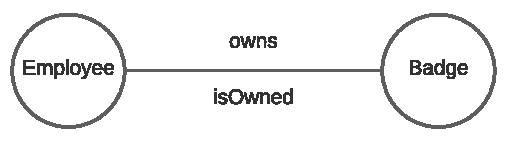
\includegraphics[width=0.5\linewidth]{immagini/one_to_one.pdf}
\caption{Connessione one-to-one.}
\label{one-to-one}
\end{figure}
\\ \\
Come mostrato in figura \ref{one-to-one} il collegamento tra i due tipi è definito come "owns" se si legge nel verso che parte da Employee per raggiungere Badge e fa riferimento all'omonimo campo di Employee. Se altrimenti la connessione si percorre nel verso opposto viene definita "isOwned", come l'omonimo campo di Badge, riportato in seguito:
\begin{verbatim}
  type Badge {
    id: ID
    isOwned: Employee
    ...
  }
\end{verbatim}
\subsubsection*{Connessione one-to-many}
In questo caso bisogna focalizzarsi sul campo \textit{worksIn} di Employee. Questo campo definisce la connessione con un elemento di tipo \textit{Department}, dunque a ciascun impiegato corrisponde un dipartimento nel quale lavora. Tuttavia pensando alla connessione in senso opposto a ciascun dipartimento possono corrispondere più impiegati. Segue dunque la rappresentazione della connessione nel grafo:\\

\begin{figure}[!h]
\centering
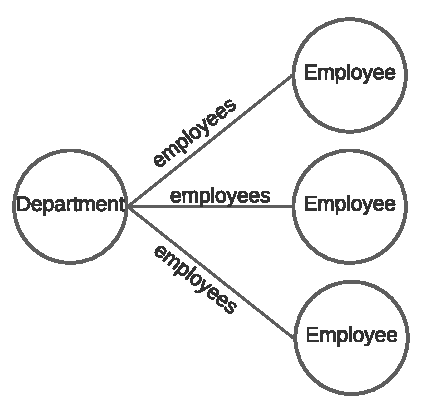
\includegraphics[width=0.4\linewidth]{immagini/one_to_many.pdf}
\caption{Connessione one-to-many.}
\label{one-to-many}
\end{figure}
\mbox{}\\
Come mostrato in figura \ref{one-to-many} il collegamento tra il dipartimento e i vari impiegati viene chiamato "employees" se si considera il verso che parte da Department per raggiungere Employee e corrisponde all'omonimo campo di Department. Tuttavia il collegamento è definito "worksIn" se la connessione viene percorsa nel verso opposto. Segue la rappresentazione del tipo Department:
\begin{verbatim}
  type Department {
    id: ID
    name: String!
    address: String!
    employees: [Employee]
  }
\end{verbatim}
\subsubsection*{Connessione many-to-many}
Consideriamo ora il campo \textit{worksOn} di Employee che collega ciascun impiegato con una lista di progetti ai quali sta lavorando. In questo caso però considerando il collegamento nel verso opposto anche ciascun progetto può avere più impiegati che ci lavorano. In questo caso si tratta di una relazione many-to-many e segue la rappresentazione nel grafo:
\begin{figure}[!h]
\centering
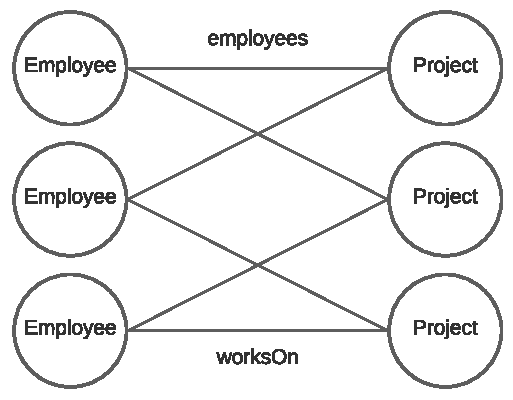
\includegraphics[width=0.4\linewidth]{immagini/many_to_many.pdf}
\caption{Connessione many-to-many.}
\label{many-to-many}
\end{figure}
\\ \\
% da sistemare questi doppi backslash
Le relazioni many-to-many non sono altro che l'unione di due relazioni one-to-many.
La connessione in questo caso, come nei casi precedenti, a seconda del verso in cui viene percorsa può esser definita come "worksOn" o "employees" come mostrato in figura \ref{many-to-many}. Di seguito la rappresentazione del tipo Project:
\begin{verbatim}
  type Project {
    id: ID
    name: String
    employees: [Employee]
  }
\end{verbatim}
\subsection*{Operazioni sui dati}
Come detto in precedenza GraphQL è un linguaggi di query e come tale permette di interrogare i dati o eseguire operazioni su di essi. Ci sono tre tipi di operazioni che possono essere fatte sui dati e queste sono: \textit{Query}, \textit{Mutation} e infine \textit{Subscription}.
\subsubsection{Query}
L'operazione di query viene utilizzata per richiedere dati da una determinata API ed equivale alla GET nel protocollo REST. È necessario dichiarare nel GraphQL schema la query che il programmatore backend desidera rendere disponibile, così facendo vengono dichiarati anche i tipi che possono eventualmente essere passati come argomenti e quelli che verranno ritornati dalla query.\\
Un esempio di dichiarazione di query che ritorna una lista di tutti gli oggetti di tipo Employee presenti in un determinato Department può essere:
\begin{verbatim}
  type query {
    employeesInDepartment(departmentId: ID!): [Employee]
  }
\end{verbatim}
In questo caso invocando la query \textit{employeesInDepartment} e passando come argomento alla query l'id (non può essere un valore nullo) del dipartimento, riceveremo come risposta un JSON contenente un campo "\textit{data}" contenente a sua volta la lista di impiegati, questo se la query ha avuto successo. In caso di insuccesso della query per qualsiasi motivo, ad esempio per avere passato un id errato, allora verrà ritornato un JSON con un campo "\textit{error}", contenente la descrizione dell'errore. \\
Dal punto di vista del client, qualora si volesse invocare questa query bisognerebbe strutturare la richiesta come segue:
\begin{verbatim}
  query {
    employeesInDepartment(id: "2BR4S") {
      id
      name
      worksOn {
        id
        name
      }
    }
  }
\end{verbatim}
Se la query non dovesse fallire, verrà ritornata una lista di impiegati e per ciascun impiegato verranno ritornati i campi specificati nella query dunque: l'\textit{id}, il \textit{name}, una lista di oggetti di tipo Project nel campo \textit{worksOn} per i quali bisognerà a loro volta specificare i campi ai quali si è interessati, in questo caso all' \textit{id} e al \textit{name} di ciascun progetto.\\
È inoltre possibile utilizzare gli argomenti delle query per controllare la quantità di dati che possono esser ritornati con un processo chiamato \textit{data paging}, oppure usarli per decidere in che ordine vogliamo che vengano ritornati i dati.
\subsubsection*{Mutation}
L'operazione di mutation viene utilizzata per eseguire modifiche sui dati. Equivale all'unione delle operazioni POST, DELETE, PUT, PATCH nel protocollo REST. Come per le query è necessario dichiarare le mutation che si voglion rendere disponibili al client.\\
Un esempio di mutation può essere:
\begin{verbatim}
  type mutation {
    addNewEmployee(employee: Employee!): Employee
  }
\end{verbatim}
In questo caso la mutation \textit{addNewEmployee} andrà ad aggiungere un nuovo impiegato nella struttura dati dell'applicativo. Il client per invocare questa mutation dovrà strutturare la richiesta come segue:
\begin{verbatim}
  mutation {
    addNewEmployee(employee: {
      name: "Mario"
    }){
      id
    }
  }
\end{verbatim}
In questa mutation è stato passato come argomento un oggetto di tipo Employee, del quale è stato specificato esclusivamente il nome (va obbligatoriamente specificato essendo un campo dichiarato non nullo). Come da definizione la mutation ritorna un oggetto di tipo Employee, del quale però in questo caso si vuole ricevere solo l'id generato. Come nel caso della query, se l'aggiunta dell'impiegato avrà successo, nel JSON di ritorno ci sarà un campo \textit{data} contenente l'id generato in seguito all' aggiunta dell'impiegato, in caso contrario sarà ritornato un JSON con un campo \textit{error} che descrive l'origine dell'errore.
\subsubsection*{Subscription}
L'ultimo tipo si chiama Subscription e si tratta di una funzione particolare resa disponibile in GraphQL, infatti grazie a questa funzione i client possono sottoscriversi ad una subscription e così facendo sarà il server ad inviare al client i dati richiesti non appena questi sono disponibili, dunque non è più necessario che sia il client a richiedere periodicamente i dati aggiornati.\\
Un esempio di definizione di una Subscription può essere:
\begin{verbatim}
  type subscription {
    newEmployeeAdded: Employee!
  }
\end{verbatim}
Il client che desidera sottoscriversi alla subscription \textit{newEmployeeAdded} dovrà mandare una richiesta strutturata come segue:
\begin{verbatim}
  subscription {
    newEmployeeAdded {
      id
      name
    }
  }
\end{verbatim}
Così facendo il server, appena viene aggiunto un nuovo impiegato, invierà direttamente al client i dati che il client ha specificato nella sottoscrizione, ovvero in questo caso l'\textit{id} e il \textit{name} dell'impiegato.\\
Essendo il server a dover inviare i dati al client e non il client che richiede i dati dal server, non è utilizzabile il protocollo HTTP per la comunicazione server - client, bisogna quindi utilizzare il protocollo WebSocket per aprire un canale di comunicazione a doppia via sopra un socket TCP.\\ \\
             % Kick-Off
% !TEX encoding = UTF-8
% !TEX TS-program = pdflatex
% !TEX root = ../tesi.tex

%**************************************************************
\chapter{Introduzione ai casi d'uso per l'analisi comparativa}
\label{cap:casi-uso}
%**************************************************************

\intro{Illustrazione del prototipo realizzato, prime considerazioni su di esso.
        Successivamente caso d'uso di SushiLab, migrazione e considerazioni.}\\
\subsection{Confronto con stakeholder}
Parlo confronto stakeholder....
\section{Prototipo}
\textcolor{red}{FORSE QUESTA PARTE VA SU UNO DEI PRIMI DUE CAPITOLI.... INTANTO LASCIO QUA.}\\\\
Prima di procedere con la spiegazione nella progettazione, realizzazione e migrazione del prototipo vanno fatte delle premesse.\\
Si tratta di un prototipo realizzato al fine di:
\begin{itemize}
  \item familiarizzare con le tecnologie Spring e Angular per la realizzazione rispettivamente di backend e frontend, il tutto in preparazione alla migrazione dell'applicativo aziendale riportato al punto \ref{sushi-lab};
  \item familiarizzare con la realizzazione delle API sia con lo stile architetturale REST, che con il linguaggio di query GraphQL;
  \item avere un caso d'uso ulteriore a conferma delle analisi che verranno poi ricavate dalla migrazione dell'applicativo SushiLab;
\end{itemize}
Per questi motivi si tratta di un prototipo specifico che mira alla realizzazione delle API e al loro massimo utilizzo.\\\\
Il prototipo che è stato scelto di realizzare è un applicazione client-server con funzione di gestionale. Deve permettere di gestire gli impiegati e i progetti ai quali stanno lavorando, il tutto in diverse sedi con diversi dipartimenti.
\subsection{Progettazione del prototipo}
\subsubsection*{Architettura generale dell'applicativo}
L'applicativo utilizza la classica architettura introdotta al punto \ref{client-server} con un backend sviluppato con Spring Boot e il frontend sviluppato con Angular. In figura \ref{prototype-architecture} è possibile visualizzare l'architettura del prototipo con API REST:
\begin{figure}[!h]
\centering
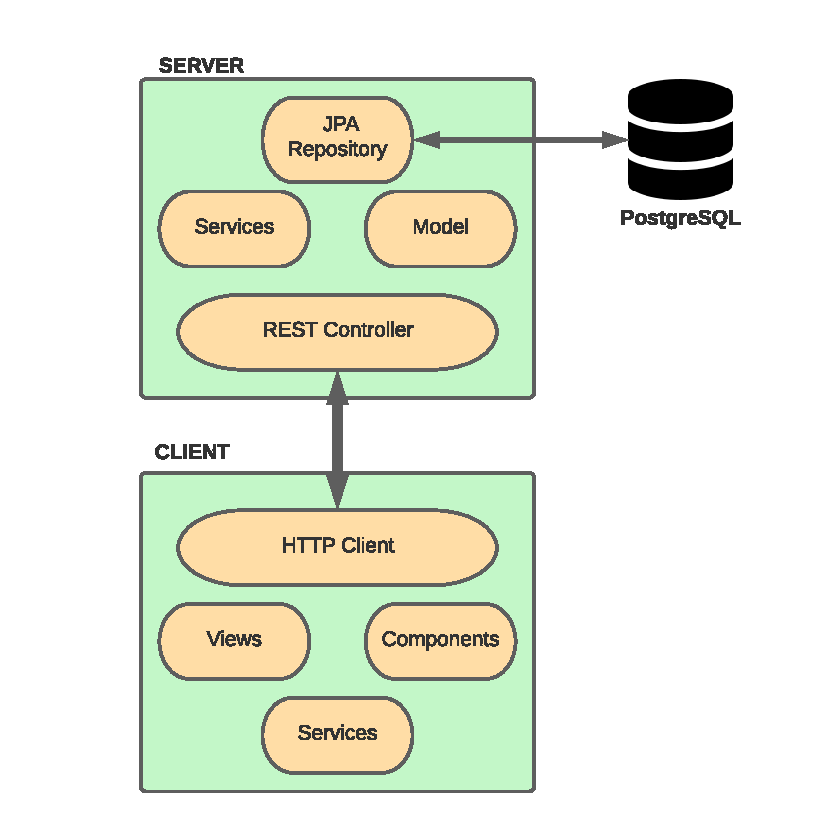
\includegraphics[width=0.6\linewidth]{immagini/prototype_architecture.pdf}
\caption{Architettura del prototipo di Web Application.}
\label{prototype-architecture}
\end{figure}
Verrà dunque realizzato un server con framework Spring Boot e la Web Application con framework Angular. Per maggiori informazioni riguardo alle tecnologie consultare il capitolo \ref{tecnologie}.
\subsubsection*{Architettura del server}
% Qui devo parlare di:
%   - pattern controller - service - repository;
%   - architettura del backend con hibernate, postgreSQL.
\paragraph{Controller - Service - Repository}
È stato deciso di seguire il pattern controller - service - repository per la realizzazione del server del prototipo. Questa scelta è stata presa in quanto è consigliato nello sviluppo del backend con framework Spring Boot. Inoltre il pattern rispetta perfettamente il principio di "Separation Of Concerns".\\
Il pattern prevedere la gestione delle entità e delle chiamate alle API attraverso tre strati:
\begin{itemize}
  \item \textbf{Controller layer}: si trova in cima all'immagine \ref{controller-service-repository}, è l'unico responsabile della interazione con entità esterne, inoltre gestisce le interfacce REST e invoca lo strato di servizio;
  \item \textbf{Service layer}: è lo strato tra controller e repository, si occupa della business logic e qualora sia necessario visualizzare, salvare, modificare o eliminare dati allora comunica con lo strato di persistenza;
  \item \textbf{Repository layer}: si tratta dello strato inferiore dell'architettura, si occupa della gestione dei dati e delle loro modifiche. Lo strato di repository inoltre si occupa della comunicazione e gestione del database.
\end{itemize}
%%%% IMG
\begin{figure}[!h]
\centering
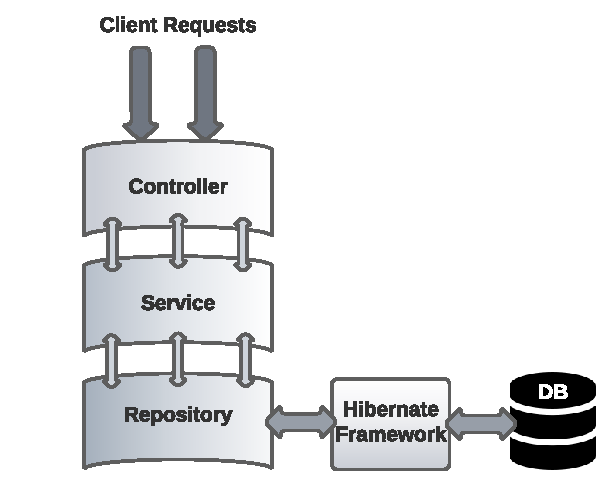
\includegraphics[width=0.8\linewidth]{immagini/controller_service_repository.pdf}
\caption{Architettura interna backend.}
\label{controller-service-repository}
\end{figure}
\textcolor{red}{PARLARE E INSERIRE QUI DIAGRAMMA DI SEQUENZA}
%%%% IMG
\paragraph{Entità e relazioni}
\label{entity-relation}
Trattandosi di un gestionale aziendale semplificato, sono previste solo quattro entità principali, queste sono:
\begin{itemize}
  \item \textbf{Employee}: l'impiegato che può lavorare ad uno o più progetti e in un dipartimento;
  \item \textbf{Project}: un progetto aziendale a cui partecipano più impiegati;
  \item \textbf{Site}: si tratta di una sede aziendale, può avere più dipartimenti;
  \item \textbf{Department}: un dipartimento che appartiene ad una sede.
\end{itemize}
%%% IMG
\FloatBarrier
\begin{figure}[!ht]
\centering
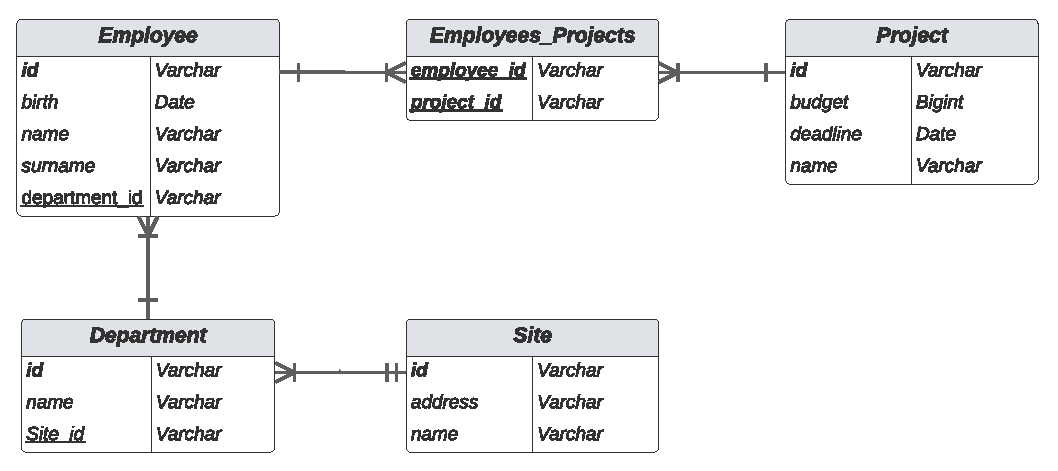
\includegraphics[width=0.8\linewidth]{immagini/ER_prototype.pdf}
\caption{Diagramma ER del prototipo.}
\label{ER-prototype}
\end{figure}
\FloatBarrier
%%% IMG
Ciascuna entità è caratterizzata da i campi presenti in figura \ref{ER-prototype} dove è stato utilizzato il linguaggio UML. Le relazioni presenti tra le varie entità sono:
\begin{itemize}
  \item \textbf{many to many}: è presente tra Employee e Project, infatti ciascun impiegato può lavorare a più progetti e ciascun progetto può avere più impiegati al quale ci lavorano;
  \item \textbf{one to many}: è presente tra due coppie di entità:
    \begin{itemize}
      \item tra Employee e Department, infatti ciascun impiegato può lavorare in uno o nessun dipartimento, mentre ciascun dipartimento può ospitare più impiegati;
      \item tra Department e Site, ciascun dipartimento può appartenere esclusivamente ad una sede, mentre ciascuna sede può esser composta da più dipartimenti.
    \end{itemize}
\end{itemize}
\subsubsection*{Realizzazione e testing server}
Durante la realizzazione viene seguito il percorso inverso rispetto a quanto visto nell'immagine \ref{controller-service-repository}, infatti la realizzazione avviene partendo dallo strato di persistenza, dunque dalla creazione delle entità e delle repositoryes.
\paragraph{Entità e repository}
A ciascun entità nel database viene fatta corrispondere una classe in Java. Per questo devono essere realizzate 4 classi rappresentanti le entità Employee, Project, Department e Site.\\
Ciascuna classe entità implementa la classe \textit{Serializable}, così facendo è possibile serializzare i dati in flussi di byte. La serializzazione viene utilizzata poiché si tratta di dati che dovranno essere memorizzati nel database, dunque è necessario serializzarli poiché abbandonano la Java Virtual Machine. Viene inoltre utilizzato un \textit{serialVersionUID} per attribuire una versione a ciascuna classe di entità serializzabile, necessario per riconoscere quando nella comunicazione con il database o con altri moduli esterni la versione dell'entità risulta differente, si tratta dunque di entità che non corrispondono totalmente, in quel caso viene ritornato un erorre \textit{InvalidClassException}.\\
Le quattro entità descritte quindi nel capitolo \ref{entity-relation} dovranno essere implementate come classi, segue l'esempio dell'implementazione della classe Employee:
%%% IMG
\FloatBarrier
\begin{figure}[!ht]
\centering
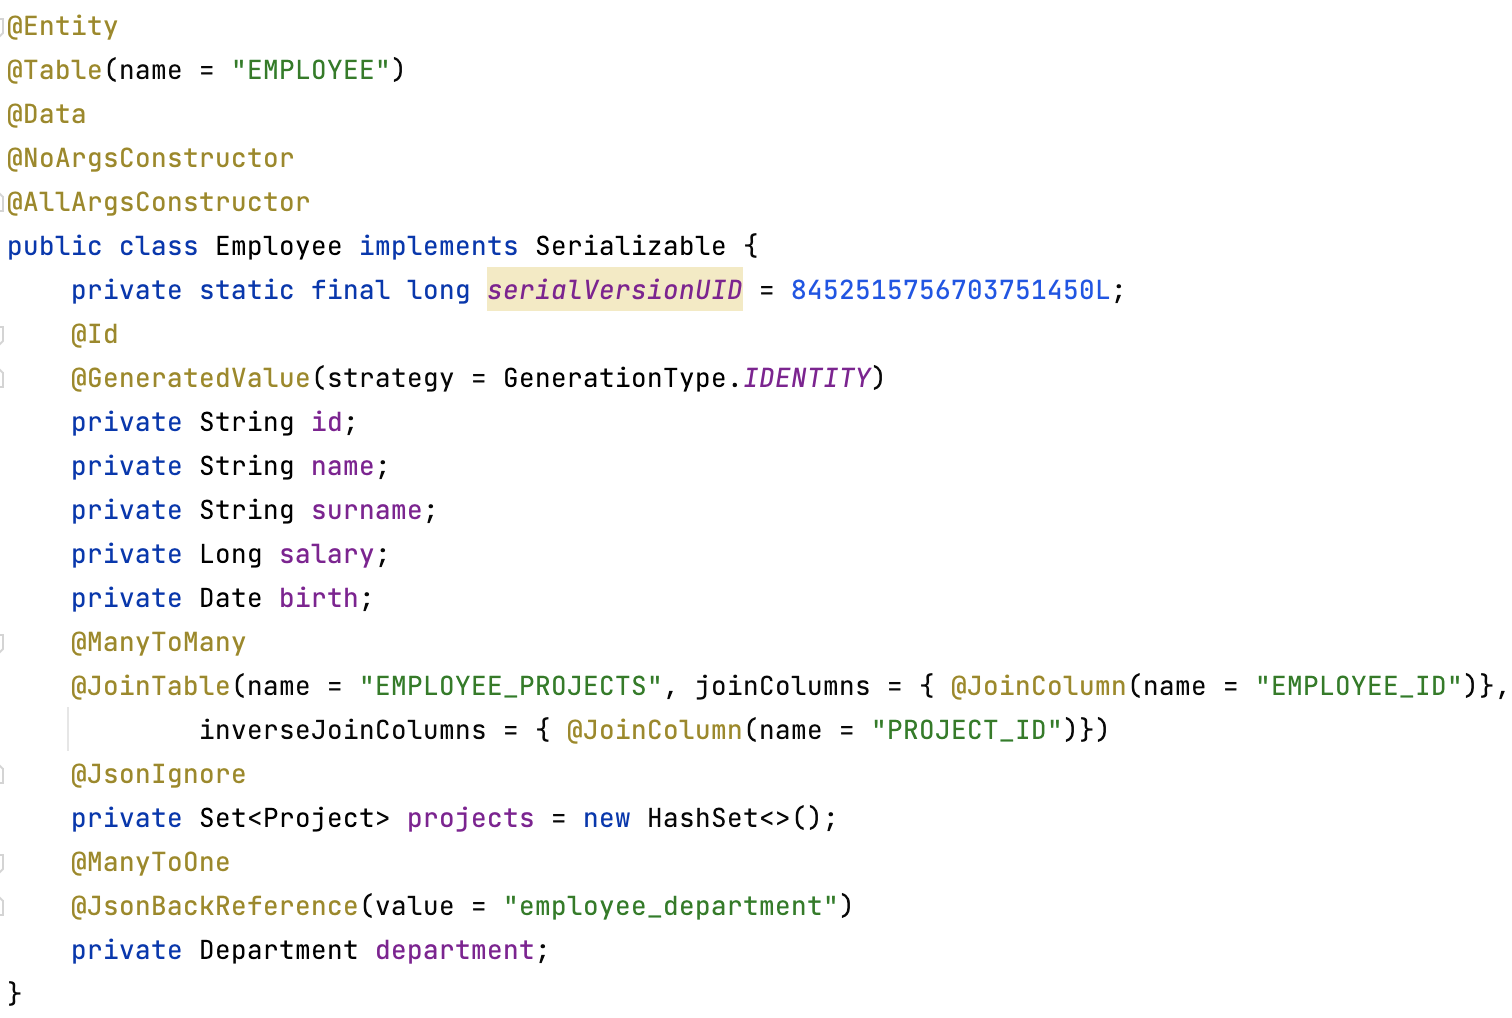
\includegraphics[width=0.9\linewidth]{immagini/employee_entity.png}
\caption{Esempio di implementazione dell'entità Employee in Spring Boot.}
\label{employee-entity-definition}
\end{figure}
\FloatBarrier
%%% IMG
Vengono attribuite alla classe Employee diverse annotazioni Spring, tra queste:
\begin{itemize}
  \item \textbf{@Entity}: si tratta dell'annotazione che permette di mappare la classe Employee come una corrispondente tabella nel database. Questa annotazione è resa disponibile dal modulo Spring Data JPA il quale implementa la specifica delle Java Persistence API attraverso Hibernate ORM e permette dunque il mapping della classi con corrispettive entità nel database;
  \item \textbf{@Table}: questa annotazione permette di specificare il  nome della tabella generata o presente nel database durante la sua creazione o aggiornamento;
  \item \textbf{@Data}: grazie alla libreria \textit{lombok} è possibile, attribuendo alla classe questa annotazione, generare automaticamente tutti i metodi get e set per tutti i campi della classe;
  \item \textbf{@NoArgConstructor e @AllArgConstructor}: permettono di generare tutti le combinazioni di costruttori con parametri e quello senza parametri.
\end{itemize}
Spostando invece il focus sui campi della classe Employee in figura \ref{employee-entity-definition}, possiamo notare che il campo \textit{id} ha due annotazioni associate. La annotazione \textbf{@Id} permette di specificare nel mapping che si tratta della chiave primaria, mentre l'annotazione \textbf{@GeneratedValue} permette di specificare che quando una nuova istanza di una entità viene creata, deve essere generato un nuovo id randomico.\\\\
Proseguendo sono presenti tutte le dichiarazioni dei vari campi dati dell'entità Employee e infine, troviamo le relazioni che Employee ha con le enetità Project e Department. Anche in questo caso le annotazioni fornite dalla specifica JPA permettono di specificare nel dettaglio le varie relazioni. Sono dunque presenti le annotazioni:
\begin{itemize}
  \item \textbf{@ManyToMany} e \textbf{@ManyToOne}: queste specificano il tipo di relazione che è presente con le altre entità, sono rispettivamente associate ai campi \textit{projects}, con il quale Employee ha una relazione molti a molti e infine al campo \textit{department}, con il quale Employee ha una relazione molti a uno;
  \item \textbf{@JoinTable}: è associata al campo \textit{projects}, e poiché le relazioni molti a molti necessitano di una ulteriore tabella per la memorizzazione di tutte le associazioni, questa annotazione permette di specificarne il nome, ovvero \textit{EMPLOYEE-PROJECTS} e i nomi delle due colonne, ovvero \textit{EMPLOYEE-ID} e \textit{PROJECT-ID};
  \item \textbf{@JsonIgnore}: associato al campo \textit{projects}, permette di escluderlo dalla serlizzazione;
  \item \textbf{@JsonBackReference}: associato al campo \textit{department}, permette di dare una direzionalità alla relazione molti a uno con Department, fondamentale per evitare il problema della ricorsione infinita \textcolor{red}{(QUI NON SO SE SPIEGARE)}.
\end{itemize}
Analogamente sono state realizzate le classi corrispondenti alle entità Project, Department e Site.\\\\
A questo punto si procede con la realizzazione delle classi repository: ciascuna entità ha una propria repository corrispondente. Dunque viene estesa l'interfaccia \textbf{JPArepository<T, ID>} con T il tipo della entità che si vuole gestire, mentre ID è il tipo della chiave primaria dell'entità T. La repository JPA deriva da diverse interfacce, tra le quali:
\begin{itemize}
  \item \textbf{CrudRepository<T, ID>}: la quale contiene le API per gestire le classiche operazioni CRUD;
  \item \textbf{PagingAndSortingRepository<T, ID>}: la quale contiene le API per gestire la pagination e il sorting;
\end{itemize}
Dunque estendendo la JPARepository per ciascun tipo è possibile avere a disposizione diversi metodi per eseguire operazioni già implementate come: findAll, count, existById, SaveAndFlush, ecc...\\
Qualora invece si volesse rendere disponibili nuovi metodi è possibile dichiararli nell'estensione della repository, senza necessariamente implementarli, poiché è sufficiente attribuire il nome corretto al metodo. Più specificatamente il nome del metodo corrispondente alla query che si vuole render disponibile è composto da un introducer che può essere uno tra: \textit{find}, \textit{read}, \textit{query}, \textit{count} o \textit{get}, e successivamente il criterio seguito dalla keywork \textit{By}, quindi ad esempio se si volesse fare una ricerca per salario, è sufficiente dichiarare un metodo chiamato \textit{findBySalary}. \\
Infine ritroviamo il caso in qui si vuole realizzare una query complessa o personalizzata, in questo caso ci viene in aiuto la annotazione \textbf{@Query} alla quale è possibile passare come attributo la query che desideriamo in linguaggio JPQL. Di seguito è possibile visualizzare quanto spiegato nell'implementazione della \textbf{EmployeeRepository} in figura \ref{employee-repository}:
%%% IMG
\FloatBarrier
\begin{figure}[!ht]
\centering
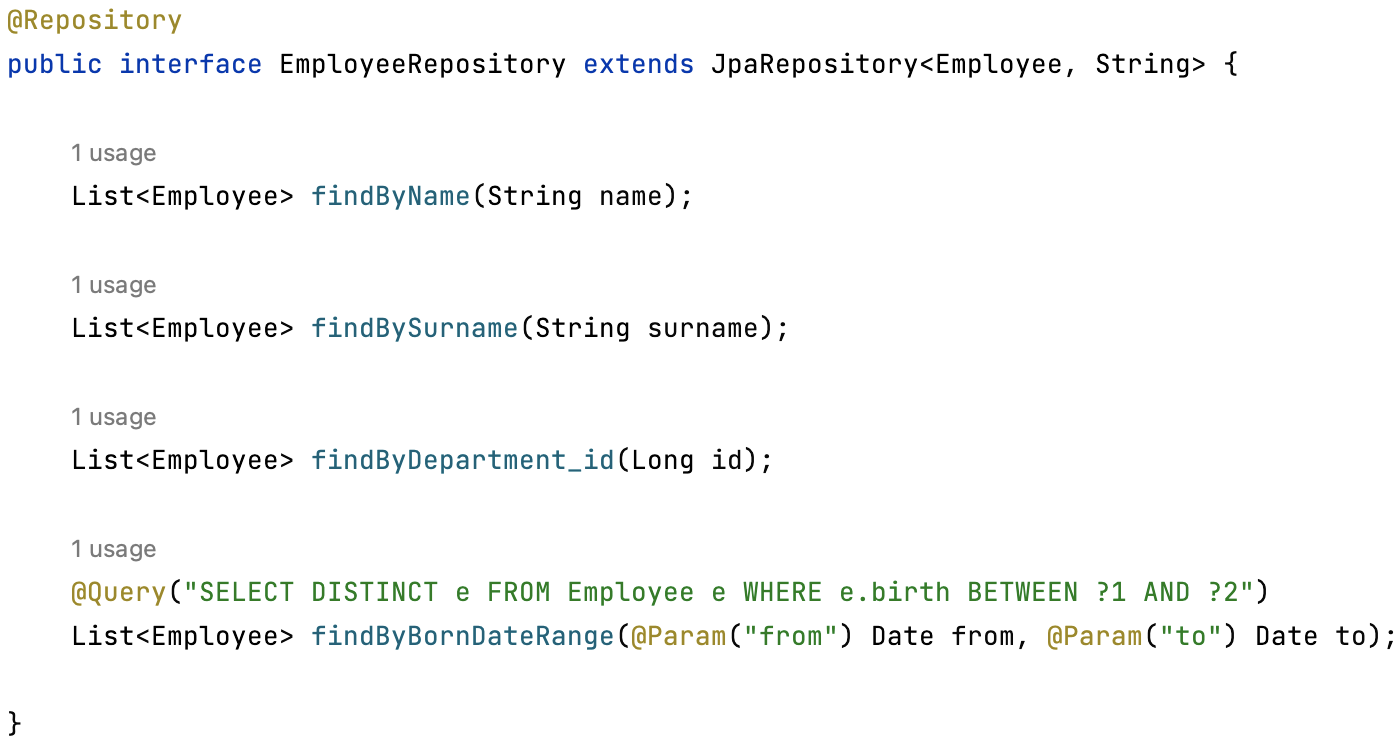
\includegraphics[width=1\linewidth]{immagini/employee_repository.png}
\caption{Esempio di implementazione della repository di Employee in Spring Boot.}
\label{employee-repository}
\end{figure}
\FloatBarrier
%%% IMG
Dunque oltre ai classici metodi di ricerca disponibili già dopo l'estensione dell'interfaccia JPARepository<T, ID>, sono stati realizzati alcuni metodi per la ricerca di impiegati per nome, per cognome e per id di dipartimento in cui lavorano. Infine è stata realizzata una query personalizzata per la ricerca di impiegati nati in un range di date.\\
Infine è possibile notare in figura \ref{employee-repository} l'annotazione \textbf{@Repository} attribuita alla'interfaccia, fondamentale al fine di indicare che la classe fornisce meccanismi per modellare i dati dell'applicativo.
\paragraph{Service}
Lo strato di servizio è lo strato che si trova tra lo strato di controller e quello di repository, il suo compito è facilitare la comunicazione tra controller e repository e inoltre contiene la business logic dell'applicativo.
Per ciascun repository, dunque per ciascuna entità, è stato realizzato un servizio specifico per gestirne le logiche.\\
Al fine di rispettare i principi SOLID della programmazione, per questioni di loose coupling e semplicità nel testing, è stato scelto di implementare il pattern secondo il quale per ogni entità viene realizzata una interfaccia del servizio ed la sua implementazione, come mostrato in figura \ref{service-serviceImpl} nel caso del servizio per l'entità Employee.
%%% IMG
\FloatBarrier
\begin{figure}[!ht]
\centering
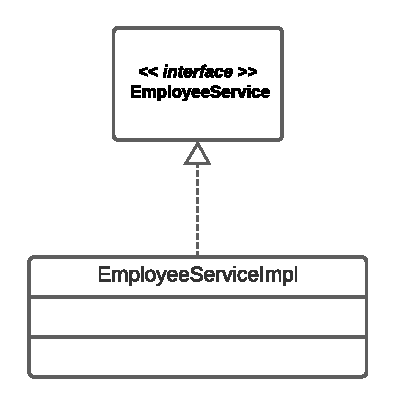
\includegraphics[width=0.3\linewidth]{immagini/service_serviceImpl.pdf}
\caption{Esempio di implementazione dell'interfaccia EmployeeService.}
\label{service-serviceImpl}
\end{figure}
\FloatBarrier
%%% IMG
Di seguito, in figura \ref{employeeServiceImpl}, viene riportato un esempio di servizio implementato, in questo caso si tratta dell'implementazione del servizio per l'Employee, ovvero della classe \textbf{EmployeeServiceImpl}.
%%% IMG
\FloatBarrier
\begin{figure}[!ht]
\begin{mdframed}
\centering
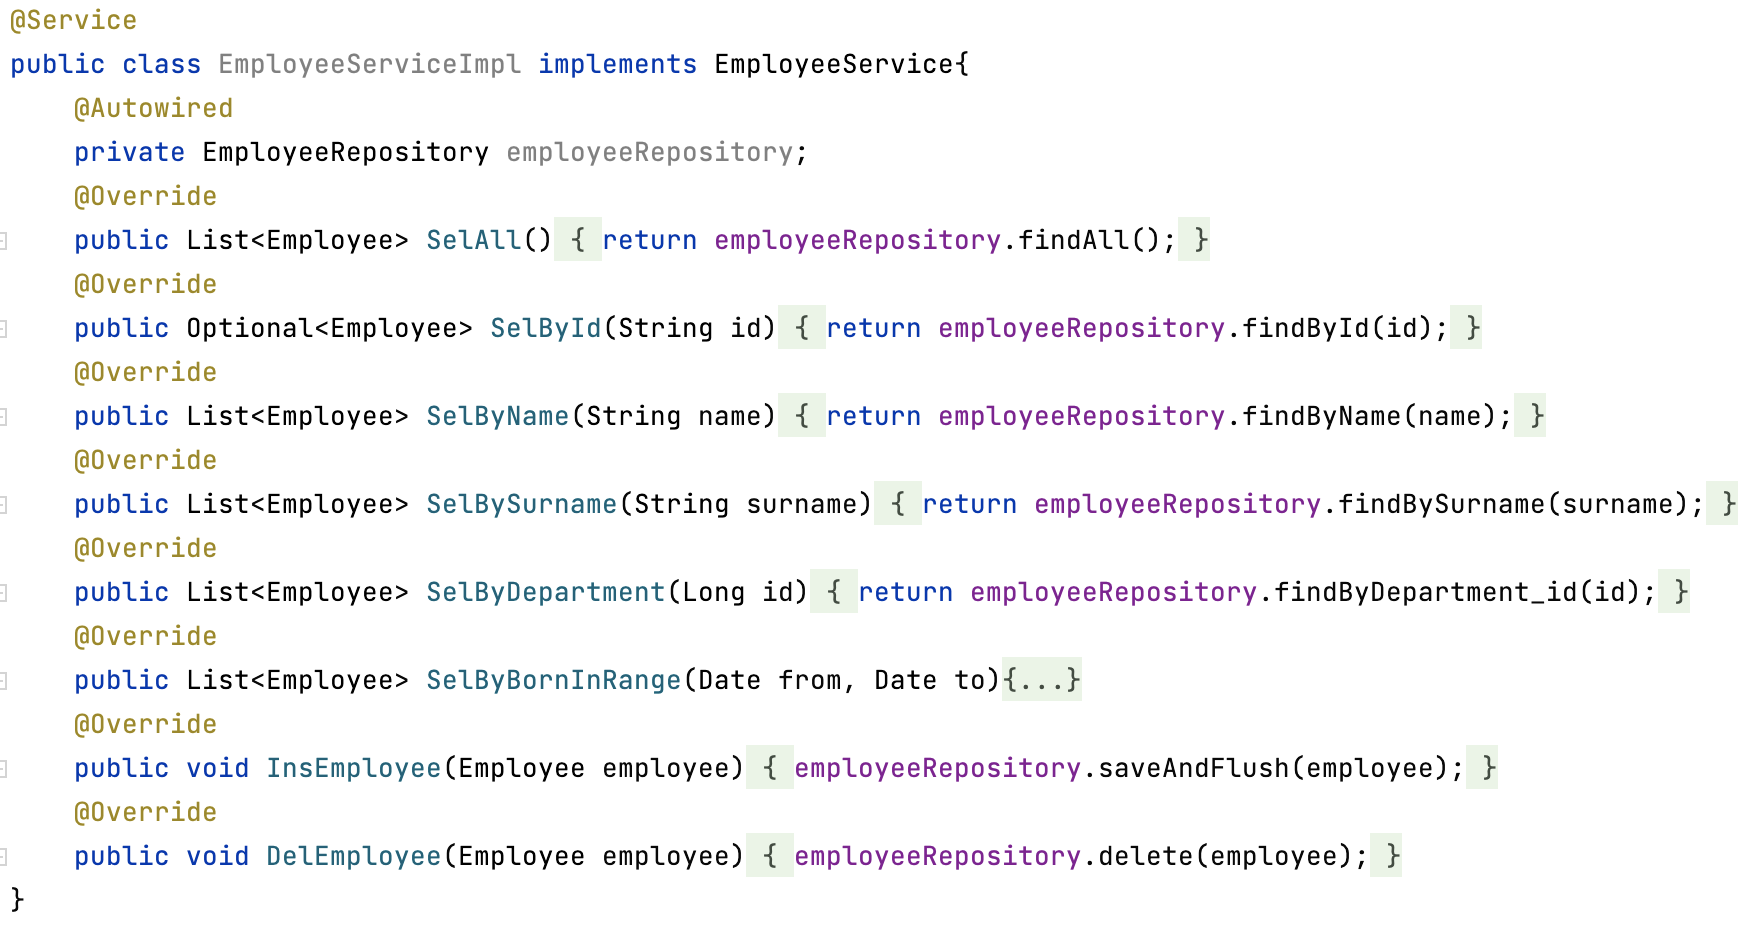
\includegraphics[width=1\linewidth]{immagini/employeeServiceImpl.png}
\end{mdframed}
\caption{Classe EmployeeServiceImpl.}
\label{employeeServiceImpl}
\end{figure}
\FloatBarrier
%%% IMG
In figura \ref{employeeServiceImpl} è possibile notare come la classe sia caratterizzata dall'annotazione \textbf{@Service} la quale viene utilizzata per indicare classi che contengono la business logic e viene utilizzata dunque per marcare la classe come service provider.\\
Continuando ed andando ad analizzare i campi dati è possibile visualizzare la dipendenza che la classe \textit{EmployeeServicImpl} ha con la repository \textit{EmployeeRepository}. In Spring questa dipendenza viene risolta con l'annotazione \textbf{@Autowired}, la quale permette di eseguire la dependency injection del bean \textit{employeeRepository}.\\
Infine sono presenti tutti i metodi, ciascuno con annotazione \textbf{@Override} poiché sono stati dichiarati anche nell'interfaccia implementata da \textit{EmployeeServiceImpl}. Sono stati resi disponibili metodi semplici che vanno ad invocare, grazie alla dipendenza con la repository, le query già disponibili con la \textit{JPARepository<T, ID>} e la query vista precedenemente \textit{SelByBornInRage}.
\paragraph{Controller}
Infine troviamo i controller, ovvero l'ultimo strato che si occupa di gestire le richieste che il server riceve attraverso il protocollo HTTP, e di mapparle inoltre ai relativi metodi. In figura \ref{employeeController} il controller di Employee, ovvero la classe \textit{EmployeeController}:
\FloatBarrier
\begin{figure}[!ht]
\begin{mdframed}
\centering
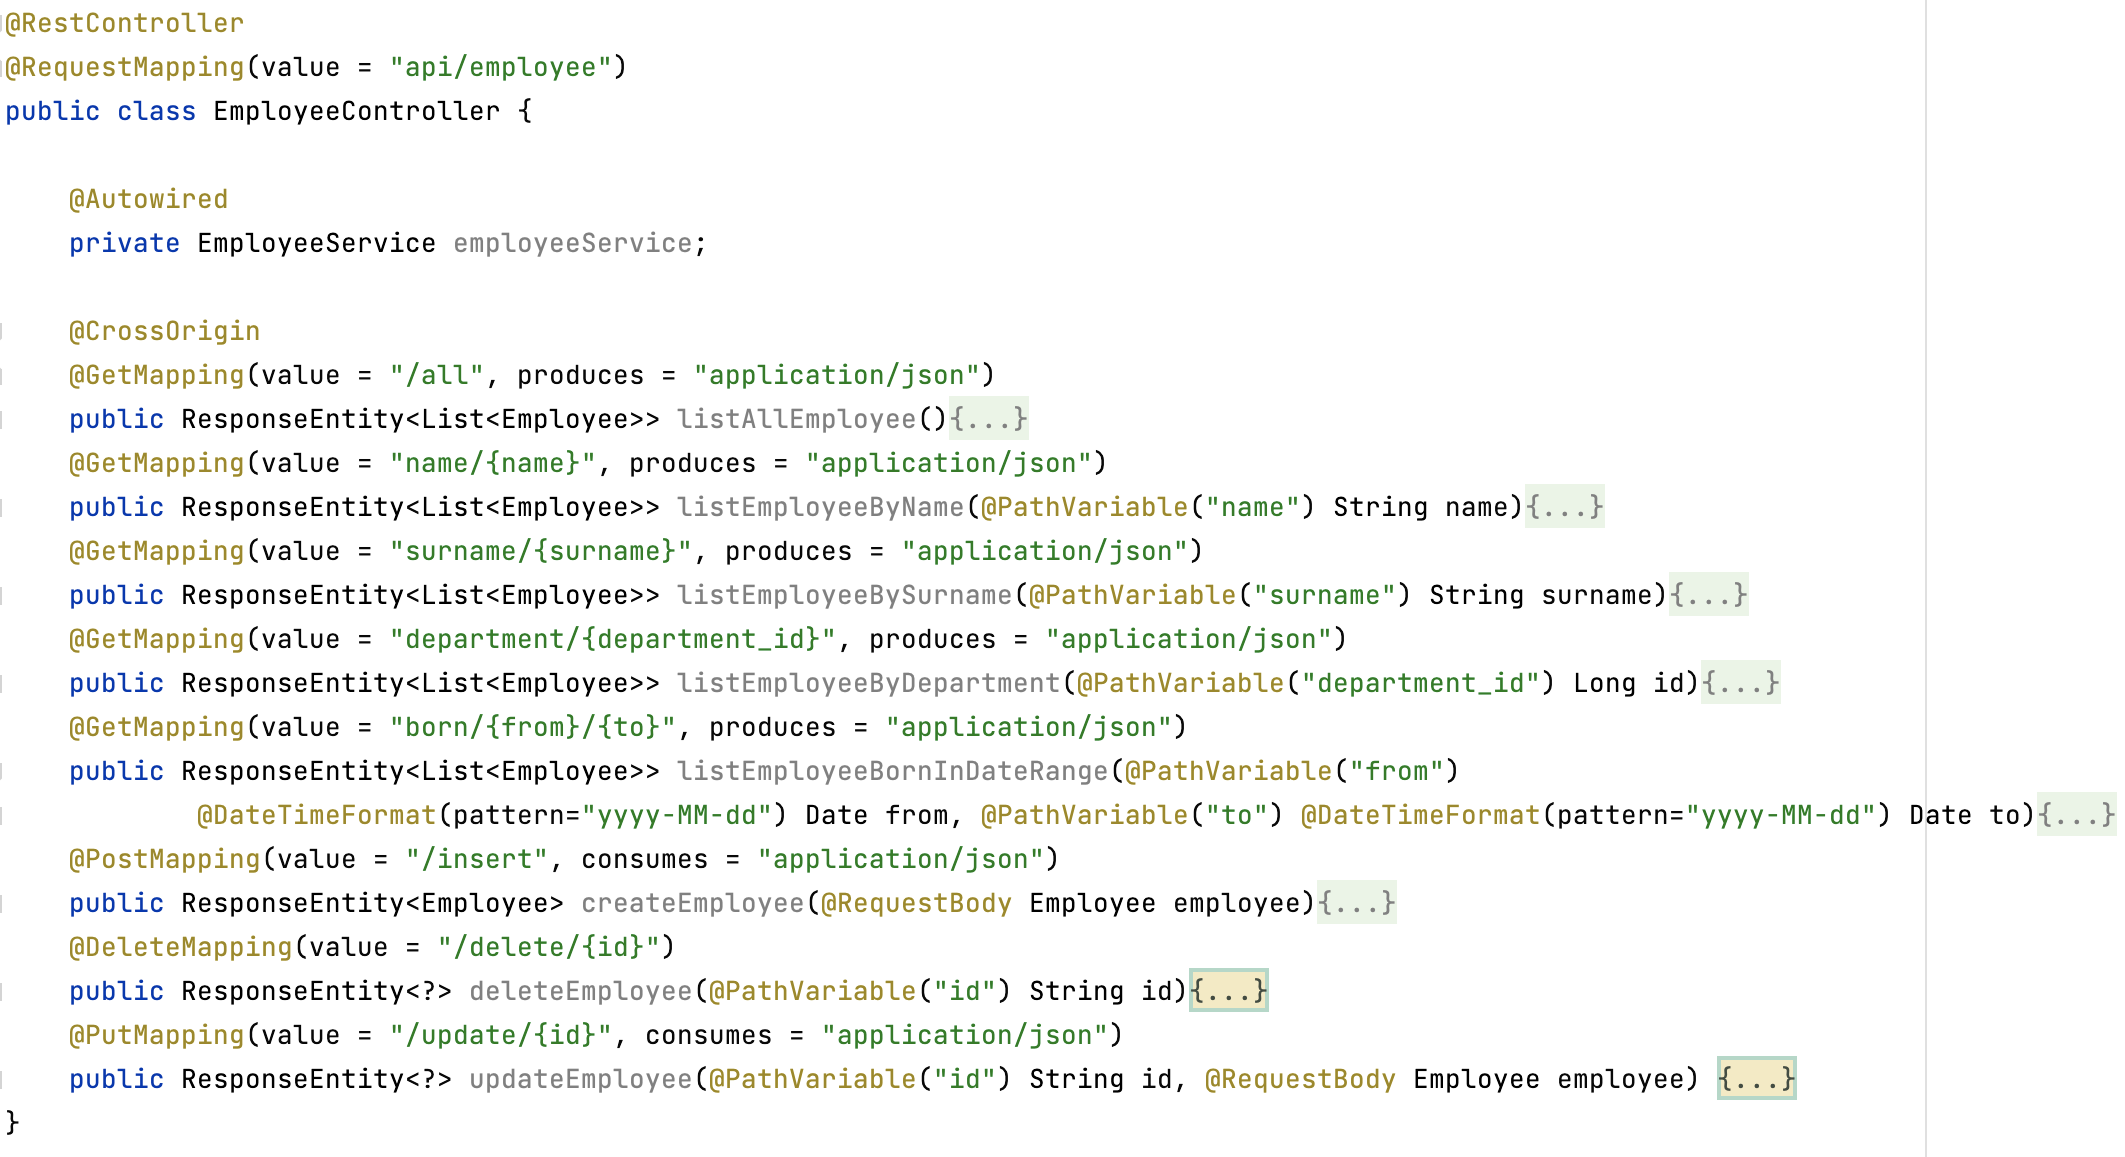
\includegraphics[width=1\linewidth]{immagini/EmployeeController.png}
\end{mdframed}
\caption{Classe EmployeeController.}
\label{employeeController}
\end{figure}
\FloatBarrier
Questa classe permette di gestire e mappare le richieste a seconda dell'url dal quale proviene la richiesta. In figura \ref{employeeController} è possibile visualizzare due annotazioni associate alla classe, l'annotazione \textbf{@RestController}, utilizzata per definire la classe come un controller di tipo REST, mentre l'annotazione \textbf{@RequestMapping} indica l'url al quale il client dovrà mandare le richieste per quello specifico controller.\\
Proseguendo è possibile indivudare una dipendenza della classe con lo strato di servizio, infatti con l'annotazione \textbf{@Autowired} e dunque con la dependency injection viene risolta la dipendenza. La classe \textit{EmployeeController} necessita una dipendenza con la classe \textit{EmployeeServiceImpl} poiché dovrà andare ad invocarne i metodi.\\
Dunque proseguendo è possibile visualizzare i vari metodi, tutti hanno una annotazione che può essere :
\begin{itemize}
  \item \textbf{@GetMapping}: indica che si tratta di un metodo per la risoluzione di una richiesta GET; specifica l'url al quale ricevere la richiesta e ciò che viene ritornato, ovvero un file JSON;
  \item \textbf{@PostMapping}: indica che si tratta di un metodo per la risoluzione di una richiesta POST, specifica l'url al quale ricevere la richiesta e ciò che richiede in input, ovvero un file JSON passato attraverso il body della richiesta HTTP;
  \item  \textbf{@DeleteMapping}: indica che si tratta di un metodo per la risoluzione di una richiesta DELETE, specifica l'url al quale ricevere la richiesta;
  \item \textbf{@PutMapping}: indica che si tratta di un metodo per la risoluzione di una richieste PUT, specifica l'url al quale ricevere la richiesta e ciò che richiede in input, ovvero un file JSON passato attraverso il body della richiesta HTTP;
\end{itemize}
Oltre alle annotazioni sopra riportate, sono presenti tra gli argomenti le annotazione \textbf{@PathVariable} la quale vuole indicare che si tratta di una variabile che verrà fornita nell'url nel posto definito dal nome specificato, \textbf{@RequestBody} ovvero un argomento che verrà fornito nel body della chiamata HTTP e infine \textbf{@DateTimeFormat} per specificare il formato del tipo di dato \textit{Date} che verrà passato dal client nell'url della richiesta.
Sono state rese dunque disponibili le seguenti query:
\begin{itemize}
  \item \textbf{listAllEmployee}: ritorna tutti gli impiegati presenti;
  \item \textbf{listEmployeeByName}: ritorna tutti gli impiegati con una determinato nome;
  \item \textbf{listEmployeeBySurname}: ritorna tutti gli impiegati con un determinato cognome;
  \item \textbf{listEmployeeByDepartment}: ritorna tutti gli impiegati di un dipartimento;
  \item \textbf{listEmployeeByBornInDataRange}: ritorna tutti gli impiegati nati in un determinato range di date;
  \item \textbf{updateEmployee}: vengono aggiornati i campi dati di un impiegato;
  \item \textbf{createEmployee}: aggiunta di un nuovo impiegato;
  \item \textbf{deleteEmployee}: rimozione di un impiegato.
\end{itemize}
\textcolor{red}{Parlare della gestione delle eccezioni con @ExceptionHandler, se ho tempo.}
\paragraph{Testing API}
Essendo un prototipo incentrato sulla realizzazione delle API, sono stati svolti in maniera semplice e veloce i test per gli strati di servizio e repository, dunque non verranno riportati. Per quanto riguarda i testi sui controller stati svolti dei test più approfonditi.\\
Per eseguire i test sui metodi del controller è stato scelto di utilizzare il framework JUnit5 \textcolor{red}{(REINDIRIZZARE AL CAPITOLO TECNOLOGIE)}.\\
Il primo test realizzato è uno \textit{SmokeTest} e da qui il nome della classe realizzata per testare che il contesto Spring abbia effettivamente creato i controller dell'applicazione. In figura \ref{smoke-test} la classe \textit{SmokeTest} con una dipendenza per ciascun controller risolta con la dependency injection grazie all'annotazione \textbf{@Autowired}. Sono poi presenti quattro metodi, uno per controller, per verificarne se sono stati creati nel contesto. Infine ciascun metodo deve essere annotato con \textbf{@Test} per indicare al framework JUnit5 che si tratta di un metodo di test.\\
Come possiamo notare sempre nell'immagine \ref{smoke-test} è presente l'annotazione \textbf{@SpringBootTest}, necessaria per indicare a Spring Boot dove si trova la principale classe di configurazione, e dunque avviare il contesto Spring. Da notare inoltre che ciascun metodo è dichiarato in maniera da poter sollevare eccezzioni se necessario.
\FloatBarrier
\begin{figure}[!ht]
\begin{mdframed}
\centering
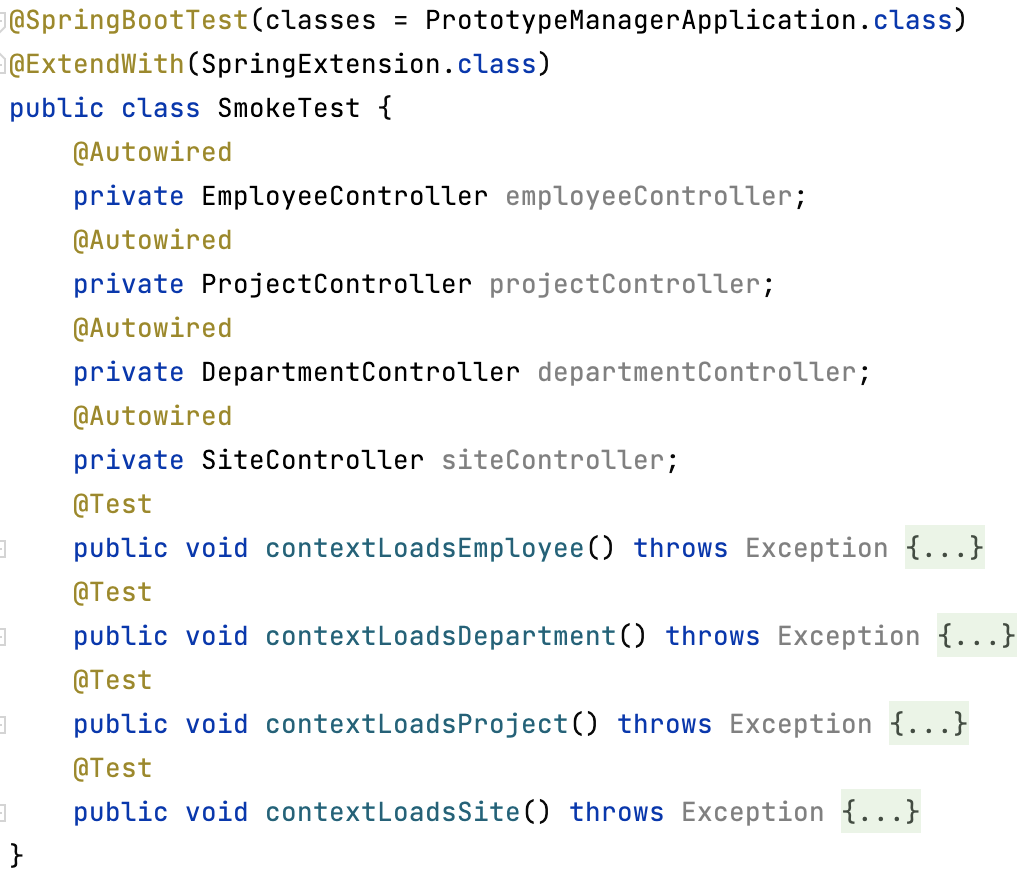
\includegraphics[width=0.7\linewidth]{immagini/SmokeTest.png}
\end{mdframed}
\caption{Classe \textit{SmokeTest} sulla creazione dei controller.}
\label{smoke-test}
\end{figure}
\FloatBarrier
Passiamo ora ai test metodi del controller \textit{EmployeeController}. Nell'immagine \ref{employee-controller-test} è raffigurata la classe \textit{EmployeeControllerTest} con metodi i vari test da effettuare sul controller.
\FloatBarrier
\begin{figure}[!ht]
\begin{mdframed}
\centering
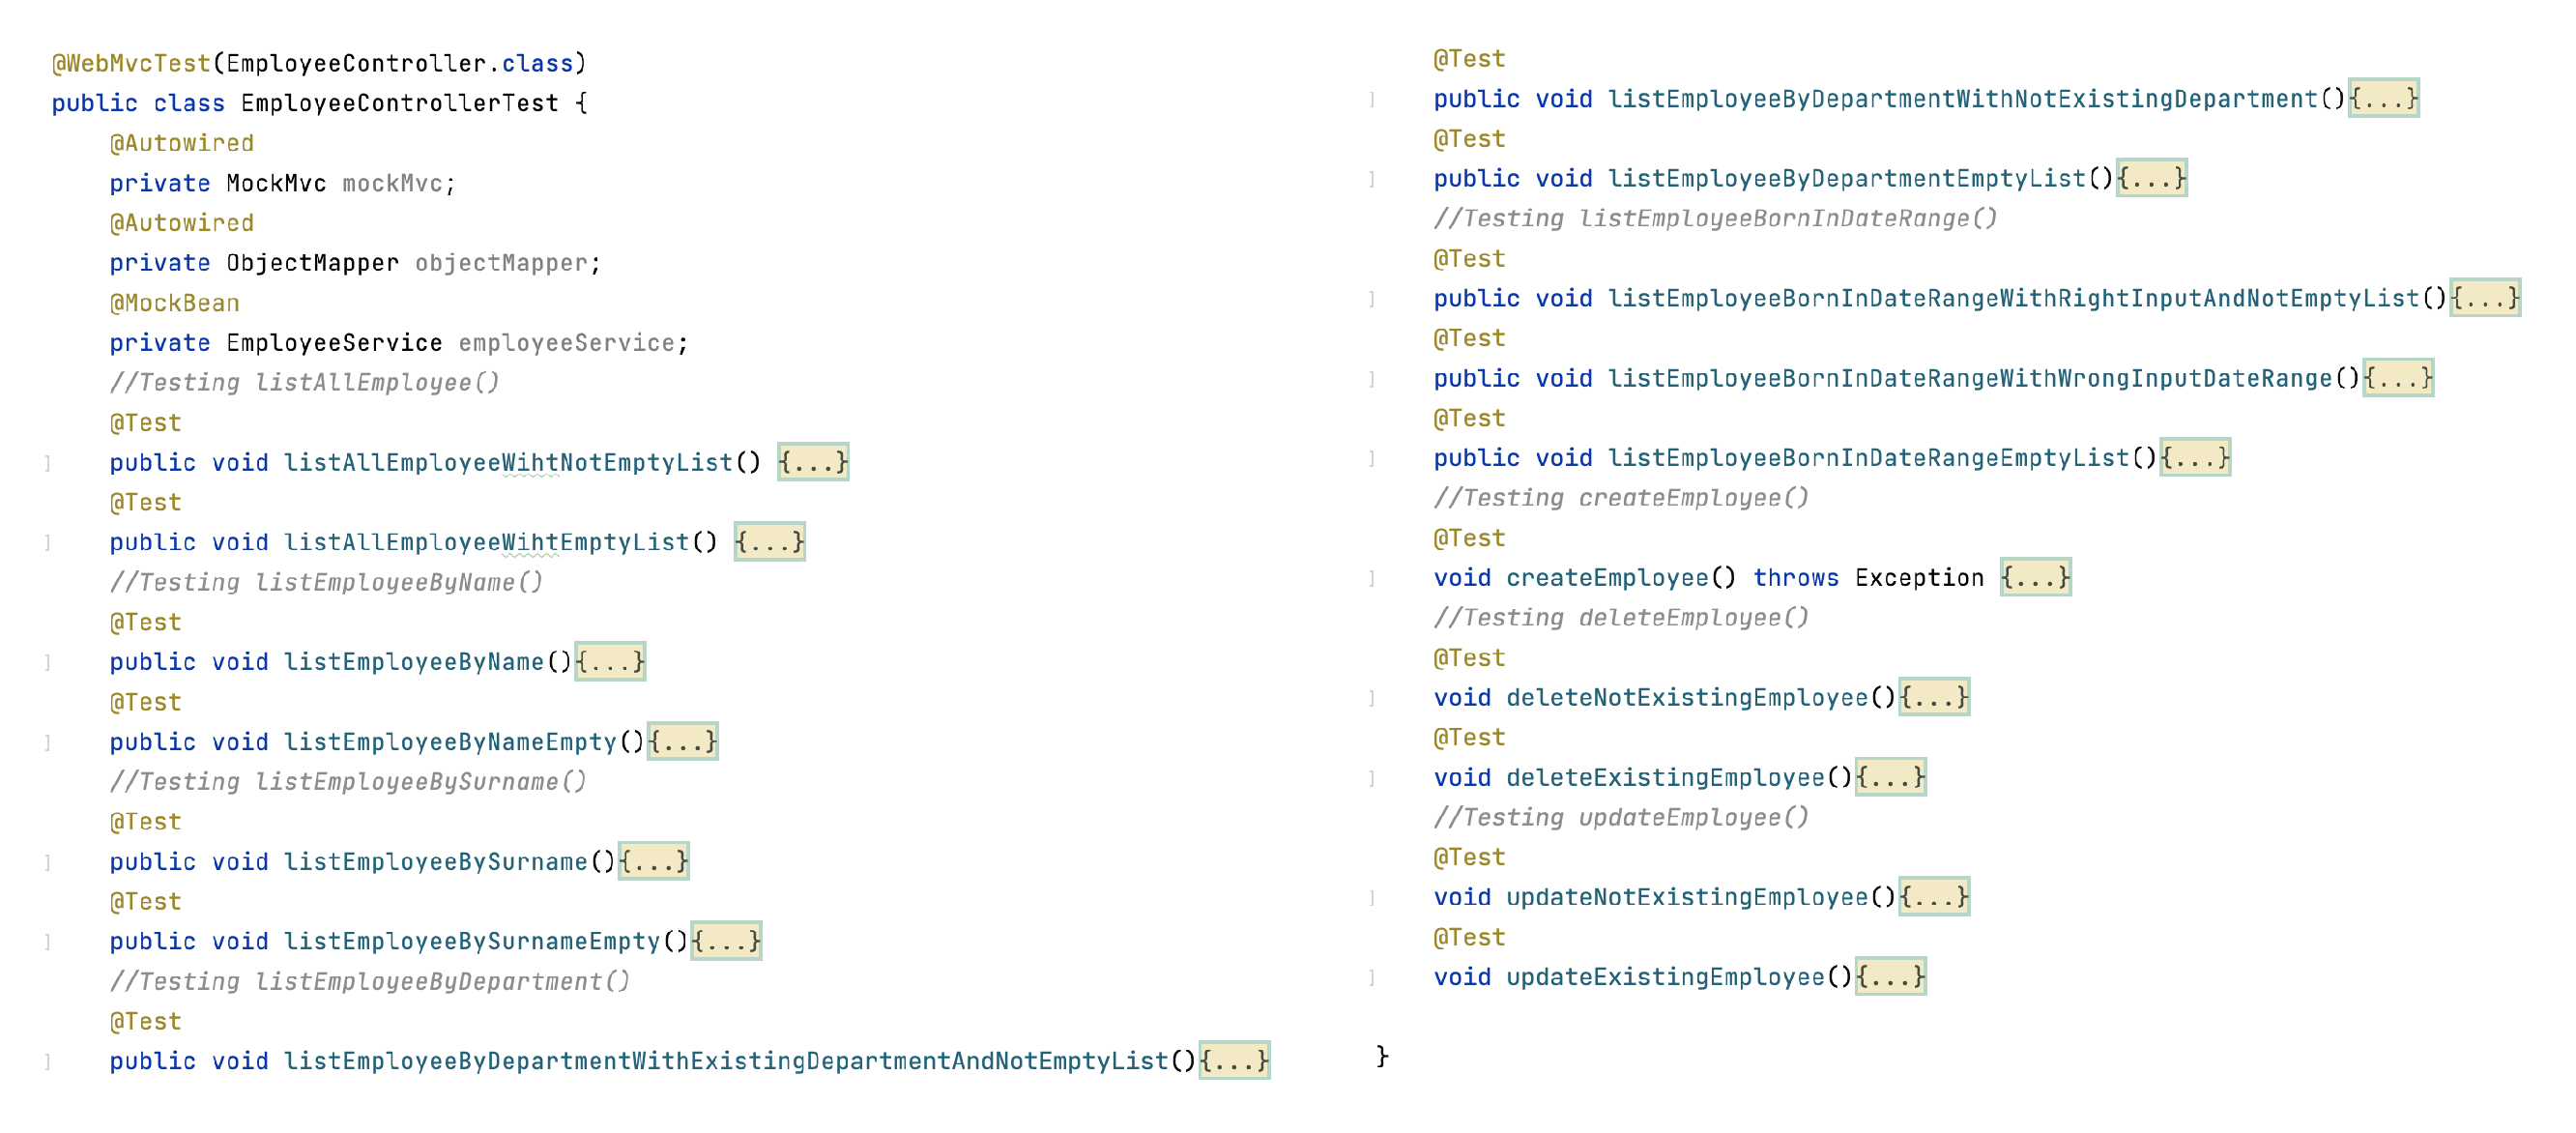
\includegraphics[width=1\linewidth]{immagini/EmployeeControllerTest.pdf}
\end{mdframed}
\caption{Classe \textit{EmployeeControllerTest}.}
\label{employee-controller-test}
\end{figure}
\FloatBarrier
Nell'immagine \ref{employee-controller-test} la classe \textit{EmployeeControllerTest} ha due annotazioni: la prima è \textbf{@WebMvcTest}, utile poiché permette di caricare nel contesto di test esclusivamente il controller di Employee e inoltre permette di tralsciare tutte le configurazioni classiche per lasciar spazio alle configurazioni di test, mentre \textbf{@ExtendWhit} permette di integrare nel contesto di test la \textit{SpringExtension} utile poiché fornisce supporto per il testing \textcolor{red}{(Non necessaria qui forse...)}.\\
Nella classe di test \textit{EmployeeControllerTest} sono dichiarate tre dipendenze fondamentali:
\begin{itemize}
  \item \textbf{MockMvc}: dipendenza risolta cona la dependency injection, viene utilizzata sucessivamente per simulare chiamate HTTP e verificarne la risposta;
  \item \textbf{ObjectMapper}: dipendenza risolta con la dependency injection, oggetto utilizzato nei test per la serializzazione e deserializzazione degli oggetti JSON in oggetti java e viceversa;
  \item \textbf{EmployeeService}: servizio che viene utilizzato nei test, per questo motivo ha l'annotazione \textbf{@MockBean}, la quale permette di aggiungere un mock dell'oggetto \textit{EmployeeService}.
\end{itemize}
Per finire la sezione sulle REST API viene di seguito riportato in figura \ref{create-employee} l'implementazione nel dettaglio del metodo di test \textit{createEmployee} seguendo il pattern \textit{Arrange - Act - Assert}.
\FloatBarrier
\begin{figure}[!ht]
\begin{mdframed}
\centering
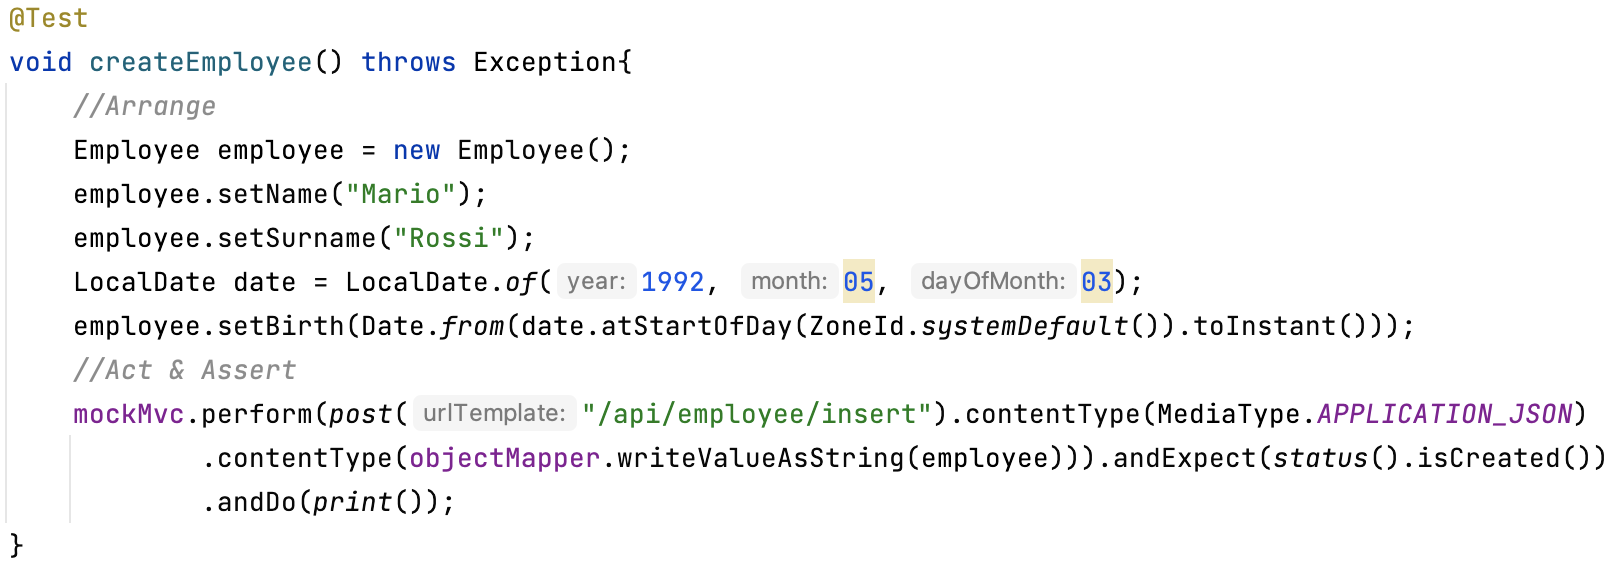
\includegraphics[width=1\linewidth]{immagini/createEmployee.png}
\end{mdframed}
\caption{Metodo di test \textit{createEmployee} della classe \textit{EmployeeControllerTest}.}
\label{create-employee}
\end{figure}
\FloatBarrier
Nella prima parte (arrange) viene creato un nuovo Employee e gli viene assegnato un nome, un cognome e una data di nascita, successivamente nella fase successiva (act), viene eseguita la chiamata GET utilizzando l'oggetto \textit{MockMvc} e passando nel body della richiesta HTTP l'oggetto Java Employee trasformato in JSON grazie all'\textit{ObjectMapper}. Infine nella fase finale (Assert), si verifica che lo stato di ritorno sia \textit{created}, in caso contrario il test fallisce.
\subsubsection*{Frontend}
Per quanto riguarda il frontend dell'applicativo è stato utilizzato il framework Angular per realizzare una single-page application. Si tratta di un frontend minimale, realizzato con il solo scopo di comprendere e sviluppare la parte di comunicazione con il server utilizzando al massimo le REST API disponibili. Per questo motivo non è stata effettuata alcuna analisi sull' utenza e sono stati tralascati completamente aspetti quali estetica grafica, accessibilità e responsive design.\\
\paragraph{Architettura}
L'architettura della web application realizzata in Angular prevede l'utilizzo del pattern Model-View-Controller:
\FloatBarrier
\begin{figure}[!ht]
\centering
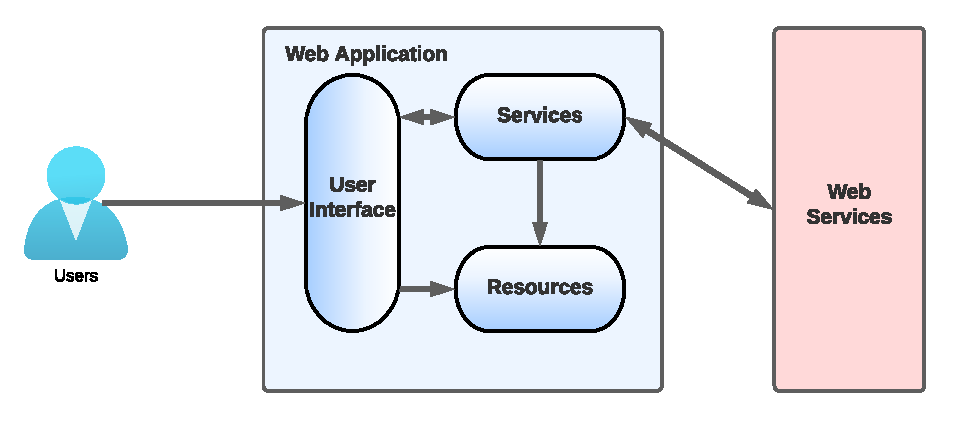
\includegraphics[width=1\linewidth]{immagini/angular_architecture.pdf}
\caption{Architettura della Web Application del prototipo.}
\label{angular-architecture}
\end{figure}
\FloatBarrier
Come visibile in figura \ref{angular-architecture} l'utente interagisce con la user interface (View) e ne modifica lo stato. Le resources (Model) vengono modificate dai services (Controller) anche su invocazione dei servizi da parte della user interface. I services sono coloro che si occupano della comunicazione con il server di backend attraverso le richiesta e risposte HTTP.
\paragraph{Funzionalità}
Per le ragioni spiegate precedentemente saranno rese disponibili nell'interfaccia grafica quelle funzionalita che andranno a permettere il massimo utilizzo delle richieste API al backend.\\
Come fatto in precedenza, verrà mostrata e spiegata esclusivamente la parte riguardante l'entità Employee per questioni di praticità, questo perché le altre entità sono state trattate in maniera analoga.\\
Dunque, in linea con le query rese disponibili dal backend riportate sulla sezione riguardante i controller, devono essere presenti le seguenti funzionalità:
\begin{itemize}
  \item \textbf{Visualizzazione degli Employee}: devono poter essere visualizzati gli impiegati in lista, o ricercati attraverso i campi: nome, cognome, data di nascita o dipartimento di appartenenza;
  \item \textbf{Aggiunta di un Employee}: deve essere possibile aggiungere un nuovo impiegato potendone specificare: nome, cognome, salario, data di nascita, dipartimento di appartenenza e infine i progetti che segue;
  \item \textbf{Aggiornamento di un Employee}: deve essere possibile aggiornare i campi dati di un impiegato specificandone l'id e il/gli campo/i da modificare;
  \item \textbf{Eliminazione di un Employee}: deve essere possibile eliminare un impiegato specificandone l'id.
\end{itemize}
Nel paragrafo sucessivo verrà mostrato come sono state implementate le funzionalità appena introdotte.
\paragraph{Implementazione FE}
Inizialmente sono state create le interfacce per poter creare gli oggetti corrispondenti alle quattro entità del prototipo. Di seguito in figura \ref{employee-interface} l'esempio della dichiarazione della interfaccia dell'entità Employee:
\FloatBarrier
\begin{figure}[!ht]
\centering
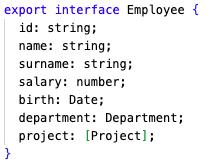
\includegraphics[width=0.3\linewidth]{immagini/employeeInterface.png}
\caption{Interfaccia di Employee.}
\label{employee-interface}
\end{figure}
\FloatBarrier
Analogamente sono state create le interfacce delle altre entità.\\
Proseguendo, è stata realizzata la realizzazione dell'interaccia grafica inserendo nella pagina iniziale la possibilità di effettuare due scelte: la prima scelta riguarda l'entità, mentre la seconda riguarda l'operazione che si vuole eseguire sull'entità selezioanta. In figura \ref{first-page} è possibile visualizzare la prima pagina:
\FloatBarrier
\begin{figure}[!ht]
\centering
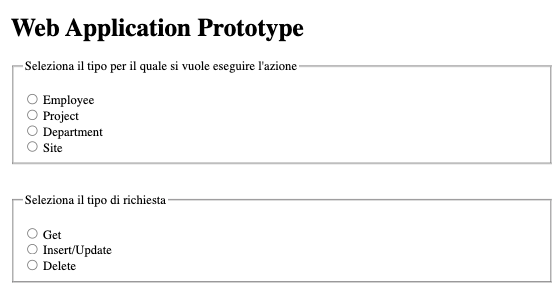
\includegraphics[width=0.7\linewidth]{immagini/firstPage.png}
\caption{Prima pagina della Web Application.}
\label{first-page}
\end{figure}
\FloatBarrier
Una volta selezionate le due opzioni viene aggiunta dinamicamente la possibilità di specificare i dettagli della richiesta. Considerando solo l'entità Employee per le ragioni spiegate precedentemente, vengono di seguito mostrate le diverse interfacce che variano al variare della scelta selezionata e il servizio che permette di eseguire la chiamata alle API del backend.\\
In figura \ref{get-employee}abbiamo il caso in cui è stato selezionata l'entità Employee con operazione GET:
\FloatBarrier
\begin{figure}[!ht]
\centering
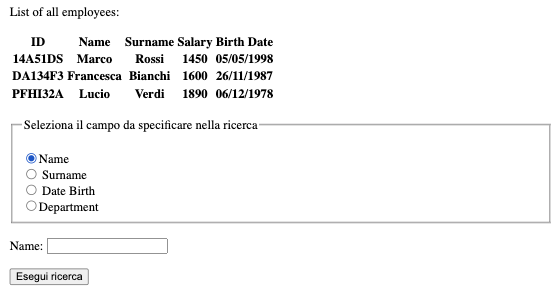
\includegraphics[width=0.7\linewidth]{immagini/getEmployee.png}
\caption{Opzioni disponibili con operazione GET selezionata.}
\label{get-employee}
\end{figure}
\FloatBarrier
Viene dunque visualizzata immediatamente una lista contenente tutti gli impiegati, per ciascun impiegato vengono mostrati id, nome e cognome, salario e data di nascita. Successivamnete viene visualizzata la scelta riguardante il campo per il quale eseguire la ricerca, in questo caso è stato scelto il nome, dunque inserendo nell'apposito campo di input il nome e selezionendo il bottone è possibile effettuare la ricerca per nome.\\
La scelta dell'opzione get permette alla vista di invocare immediatamente il servizio che esegue una chiamata alle REST API del backend per ricevere la lista di tutti gli employee, stessa cosa accade anche quando premiamo il bottone "Esegui ricerca " dopo aver inserito il nome. Il servizio in questione si chiama \textit{EmployeeService} e di seguito in figura \ref{employee-service} ne è riportata l'implementazione:
\FloatBarrier
\begin{figure}[!ht]
\centering
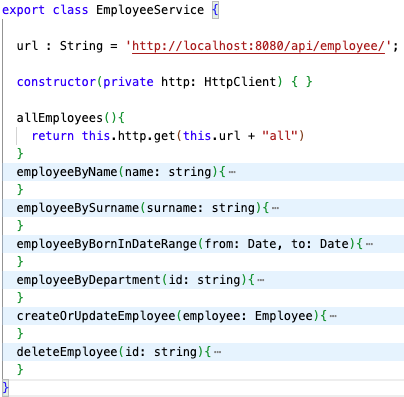
\includegraphics[width=0.6\linewidth]{immagini/employeeService.png}
\caption{Classe \textit{EmployeeService}.}
\label{employee-service}
\end{figure}
\FloatBarrier
Il servizio realizzato per le chiamate alle REST API del backend, permette di essere invocato direttamente dalla vista alla selezione di un elemento HTML.\\\\
Proseguendo verranno visualizzati ora i casi in cui si sceglie come operazione quella di modificare o aggiungere un nuovo impiegato. In figura \ref{insert-update} è possibile visualizzare la porzione di interfaccia grafica per l'inserimento o l'aggiornamento di un impiegato:
\FloatBarrier
\begin{figure}[!ht]
\centering
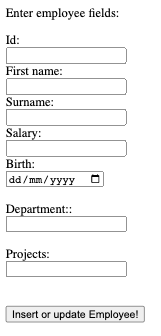
\includegraphics[width=0.3\linewidth]{immagini/postEmployee.png}
\caption{Opzioni disponibili con operazione Insert/Update selezionata.}
\label{post-employee}
\end{figure}
\FloatBarrier
Dunque una volta inseriti tutti i valori per ciascun campo, tranne il campo ID che viene generato automaticamente, è possibile aggiungere un nuovo impiegato. Qualora invece si specificasse anche l'id, allora si tratterebbe di una modifica di un employee già esistente, questo solo se l'id inserito corrisponde veramente all'id di un employee. Anche in questo caso selezionando il bottone "Insert or update Employee!" viene invocato il metodo del servizio riportato in figura \ref{employee-service}.\\
Per finire in figura \ref{delete-employee} il caso in cui venga selezionata l'opzione delete:
\FloatBarrier
\begin{figure}[!ht]
\centering
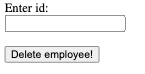
\includegraphics[width=0.3\linewidth]{immagini/deleteEmployee.png}
\caption{Opzioni disponibili con operazione Delete selezionata.}
\label{delete-employee}
\end{figure}
\FloatBarrier
%Come è stato realizzato il FE del protitipo: main components, strato servizio (con chiamate alle API del BE), ecc...
%Desing pattern adottati (ad es. MVC, Dependency Injection, principi SOLID, Signleton, ecc...).
\paragraph{Testing FE}
Spiegazione su come vengono realizzati i test sulle API call al BE.







\subsection{Migrazione da REST a GraphQL}
\subsubsection*{Migrazione Backend}
Spiego come è stata realizzata la migrazione da REST a GraphQL. Partendo da backend, viene realizzata un'analisi sui tipi necessari da riportare nel GraphQL schema (tipi di input e tipi di ritorno). Sucessivamente vengono ristrutturate le API rese disponibili in REST (non sempre i metodi dei controller REST corrispondono a quelli GraphQL, oltre a differenze nelle annotazioni, ecc...). Vengono dunque implementati i metodi dei controller GraphQL, soffermarsi sulle difficoltà riscontrate nel mapping dei tipi GraphQL schema con i tipi corrispondenti del BE. Una volta ricostruito tutto il sistema di query GraphQL nel BE e testato, si può passare alla migrazione frontend. Volendo dividere il tutto in subsubsection:
\begin{itemize}
  \item analisi sui tipi;
  \item ristrutturazione API secondo principi GraphQL;
  \item realizzazione API con tool Spring GraphQL (e problemi mapping tipi);
  \item testing;
\end{itemize}
\subsubsection*{Migrazione Frontend}
La migrazione su FE è molto più semplice rispetto al BE, infatti è sufficiente andare ad aggiornare lo strato di servizio, il quale si occupa della gestione della chiamate API al BE. Anche qui si possono riscontrare alcuni problemi per quanto riguarda la corrispondenza dei tipi (ma ho avuto più problemi in SushiLab, qui trascurabile dunque).
Volendo dividere il tutto in subsubsection:
\begin{itemize}
  \item aggiornamento strato servizio con modulo apollo;
\end{itemize}
Questo capitoletto conterrebbe tutto, da come costruire la query a seconda di ciò che è necessario, all'eliminazione della parte di gestione delle risorse nel protitipo REST (per questioni di under e overfetching).

\section{SushiLab}
\label{sushi-lab}
\subsection{Comprensione dell'applicativo}
Breve panoramica su SushiLab, ambito d'uso, funzionalità, ecc...
\subsubsection{Panoramica del backend}
Panoramica su architettura del backend (sviluppato in Spring), entità e relazioni, business logic, strato di persistenza, test, \textbf{API} (Parte preponderante della panoramica sul backend).
\subsubsection{Panoramica del frontend}
Panoramica su architettura del frontend (sviluppato in Angular), principali components, \textbf{strato di servizio} (parte preponderante perché gestisce le chiamate alle API del backend).
\subsection{Migrazione del BE da REST a GraphQL}
Molto simile a quanto scritto per il prototipo nella parte di migrazione adattato alle API specifiche di SushiLab.
\subsection{Migrazione del FE da REST a GraphQL}


% \subsection{Progettazione }
% Tecnologie scelte per lo sviluppo del protitipo (poi espresse meglio in capitoli successivi).
% Viene spiegata l'architettura del software che si vuole realizzare (diviso per BE e FE), le entità e relative relazioni.
% \subsection{Business logic - BE}


% \subsection{Sviluppo API}
% Panoramica su quali api vengono rese disponibili da BE.
% \subsubsection{Sviluppo REST API}
% Come vengono implementate con protocollo REST.
% \subsubsection{Sviluppo GraphQL API}
% Come vengono implementate con protocollo GraphQL.
% \subsection{Comparazione dei due protocolli}
% Illustrazione delle differenze (con vantaggi e svantaggi) individuate nelle varie fasi di realizazzione del
% prototipo (analisi, progettazione, sviluppo, testing, ...). Si tratta di:
% \begin{itemize}
%         \item differenze architetturali del prototipo (dunque come sono strutturati BE e FE a seconda della tecnologia utilizzata, differenze lievi ma presenti);
%         \item differenze legate alla natura dei protocolli (ad es. che GraphQL non usa i codici di stato http classici),dunque come si rispecchiano queste differenze nel concreto (ad es. gestione differente degli errori) ;
%         \item differenze negli strumenti utilizzati (ad es. differenti librerie).
% \end{itemize}
% \section{SushiLab}
% \subsection{Comprensione della struttura e delle logiche della webapp}
% Descrizione di BE e FE della webapp, sue entità, relazioni e logica di base.
% \subsection{Migrazione BE da REST a GraphQL}
% \subsubsection{Analisi delle componenti da modificare}
% Ad esempio i metodi i controller.
% \subsubsection{Realizzazione della migrazione}
% Come ogni componente varia durante tutta la migrazione.
% \subsubsection{Difficoltà riscontrate durante la migrazione}
% Problemi riscontrati nel passaggio da REST a GraphQL (ad es. problemi legati alla forte tipizzazione di GraphQl).
% \subsection{Migrazione FE da REST a GraphQL}
% Stessa cosa del BE, probabilmente sarà molto più breve.
% \subsubsection{Analisi delle componenti da modificare}
% \subsubsection{Realizzazione della migrazione}
% \subsubsection{Difficoltà riscontrate durante la migrazione}
% \subsection{Analisi comparativa}
% Analisi comparativa della webapp nelle due versioni. Vantaggi e svantaggi della webapp due versioni sotto tutti i punti di vista:
% \begin{itemize}
%         \item complessità dei protocolli e dunque i costi per la realizzazione di una versione rispetto all'altra;
% \end{itemize}


% Volendo aggiungo anche un analisi prestazionale riportando i risultati del load testing.
% \subsection{Considerazioni finali}
% Perché in questo caso d'uso specifico ha più senso utilizzare un protocollo rispetto che l'altro.
             % Concept Preview
% !TEX encoding = UTF-8
% !TEX TS-program = pdflatex
% !TEX root = ../tesi.tex

%**************************************************************
\chapter{Analisi comparativa dei protocolli REST e GraphQL}
\label{cap:analisi-comparativa}
%**************************************************************
\intro{In questo capitolo verrà svolta l'analisi comparativa tra i due protocolli REST e GraphQL, sia dal punto di vista teorico che da quello pratico .}\\
%**************************************************************
%\section{Analisi comparativa teorica}
%\label{sec:analisi-comparativa-teorica}
%Per analisi comparativa teoria s'intende tutti quegli aspetti che differenziano i due protocolli GraphQL e REST
\section{Introduzione}
REST è stato ed è tutt'oggi lo standard più seguito per la realizzazione delle Web API, tuttavia dopo l'uscita di GraphQL gli sviluppatori hanno iniziato ad utilizzare sempre di più la nuova tecnologia. Infatti GraphQL ha portato con se delle interessanti soluzioni per molti dei problemi e dei vincoli dello stile architetturale REST.\\
L'innovazione portata da GraphQL è stata apprezzata in larga scala tra gli sviluppatori, a conferma di ciò è possibile visualizzare nell'immagine \ref{graphQL-usage-chart} l'aumento nell'utilizzo di questa tecnologia con il passare degli anni.
\FloatBarrier
\begin{figure}[!ht]
\centering
\includegraphics[width=1\linewidth]{immagini/GraphQLUsageChart.png}
\caption{Grafico sull'utilizzo di GraphQL negli anni.}
\label{graphQL-usage-chart}
\end{figure}
\FloatBarrier
Nel seguente capitolo verranno analizzati nel dettaglio e paragonati i due protocolli, sotto tutti i punti di vista, mettendo in risalto vantaggi e svantaggi di ciascuno; infine verranno riportate le deduzioni elaborate durante lo stage sul protocollo che è meglio seguire in base all'applicativo che si vuole sviluppare.
\section{Analisi comparativa}
Come sottolineato in precedenza, GraphQL e REST hanno diversi aspetti che li differenziano. La più grande differenza tra questi due protocolli è legata alla loro natura: infatti quando si fa riferimento a REST, si sta parlando di uno stile architetturale, dunque di un modo di costruire le proprie API le quali, se rispettano i vincoli REST illustrati al punto \ref{principi-REST}, vengono definite RESTful. Quando si fa riferimento a GraphQL invece, si sta parlando di un linguaggio di query fortemente tipizzato.\\\\
Di seguito è presente un'analisi comparativa dettagliata per ciascun aspetto che differenzia i due protocolli di data fetching.
\subsection{Endpoints}
La prima grossa differenza tra i due protocolli riguarda gli endpoint.\\
Lo stile REST prevede l'utilizzo di più endpoint, sfrutta infatti la molteplicità degli endpoint per differenziare le richieste possibili. Quando un client implementa una richiesta a delle REST API deve sapere esattamente a quale endpoint inviare la richiesta per ricevere i dati necessari. In figura \ref{REST-endpoints} viene rappresentato la struttura degli endpoint multipli di un REST server con il client che invia diverse richieste ai diversi endpoint.
\FloatBarrier
\begin{figure}[!ht]
\centering
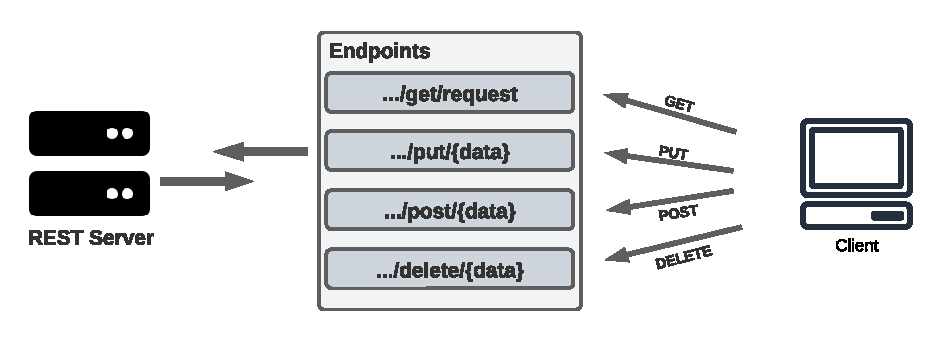
\includegraphics[width=1\linewidth]{immagini/RESTEndpoints.pdf}
\caption{Gli endpoints multipli in REST.}
\label{REST-endpoints}
\end{figure}
\FloatBarrier
Con GraphQL questo non avviene, infatti GraphQL prevede l'esposizione di un unico endpoint. A questo singolo endpoint possono essere inviate tutte le richieste inserendo nel body della richiesta la query, la mutation o la subscription. In figura \ref{GraphQL-endpoint} è possibile visualizzare come il GraphQL server fornisca un unico endpoint e come il client invii tutti i tipi di richieste allo stesso medesimo endpoint.
\FloatBarrier
\begin{figure}[!ht]
\centering
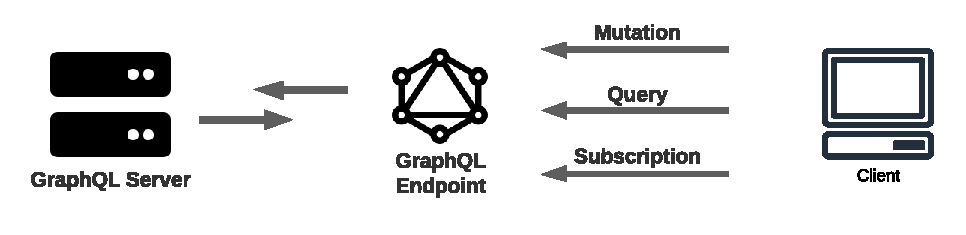
\includegraphics[width=1\linewidth]{immagini/GraphQLEndpoint.pdf}
\caption{Il singolo endpoint GraphQL.}
\label{GraphQL-endpoint}
\end{figure}
\FloatBarrier
A proposito di ciò viene riportata di seguito una citazione di Lee Byron, il co-creatore di GraphQL:
\begin{quoting}
  \textit{"Think in graphs, not endpoints."}
\end{quoting}
\subsection{Overfetching e Underfetching}
La questione dell'overfetching e underfetching è uno degli aspetti che viene maggiormente considerato nella decisione architetturale riguardo quale protocollo di data fetching utilizzare tra REST e GraphQL.\\
Lo stile architetturale REST non prevede di definire lato client esattamente quali dati ricevere. Un client che necessita un certo insieme da un server con REST API, è costretto ad eseguire una o più richieste e dunque a prendersi in carico della rielaborazione dei dati. Per uno sviluppatore backend è molto complesso riuscire a creare delle REST API che siano in grado di soddisfare esattamente le tutte le richieste dei client.
L'introduzione di GraphQL come nuovo protocollo di data fetching ha posto una soluzione a questo problema, permettendo al client di specificare esattamente la forma e il quantitativo di dati necessari. Quando si decide di implementare un applicativo e si valuta quale protocollo di data fetching utilizzare, questo è sicuramente un punto da considerare.\\
\paragraph{Overfetching}
Quando si parla di overfetching si fa riferimento al fatto che vengano forniti più dati di quanti realmente necessari. Riprendendo come esempio il prototipo visto nel capitolo \ref{casi-uso}, si suppone che il client necessiti della lista degli impiegati e che, per ciascun impiegato, necessiti  esclusivamente l'id e il nome. Qualora si tratti della version REST del server, il client inviare la richiesta HTTP all'endpoint mappato sul metodo \textit{allEmployee()}, il quale ritorna una lista di impiegati e, per ciascun impiegato, tutti i campi. Di seguito il JSON di risposta che il client riceve in seguito alla richiesta nel caso in cui fossero presenti solo due impiegati:
\begin{verbatim}
  [
    {
        "id": "3AFASDF12F",
        "name": "Matteo",
        "surname": "Verdi",
        "salary": 1500,
        "birth": "1995-02-21"
    },
    {
        "id": "GA14PL3FAV",
        "name": "Marco",
        "surname": "Blu",
        "salary": 1500,
        "birth": "1993-12-20"
    }
  ]
\end{verbatim}
Si può subito notare come i campi \textit{surname}, \textit{salary} e \textit{birth} non siano necessari in quanto il client utilizza solo i campi \textit{id} e \textit{name}. Nel caso del prototipo si tratta di un problema irrisorio data la ridotta grandezza dei dati, tuttavia in applicativi a larga scala che richiedono grossi quantitativi di dati complessi può risultare un problema in termini di occupazione di rete e di rallentamenti dell'applicativo. Questo problema può essere risolto in un server con REST API fornendo endpoint specifici per ciascun tipo di richiesta, tuttavia questa soluzione rischia di introdurre confusione e nel tempo la manutenzione potrebbe risultare sempre più complessa.\\
GraphQL risolve questo problema attribuendo al client la responsabilità di definire quali siano i campi di cui necessita. Questo è possibile specificando nella query i campi richiesti, di seguito l'esempio dell'invocazione contenente a sinistra la query \textit{allEmployees}, mentre a destra il JSON ricevuto in risposta:
\begin{verbatim}
    QUERY                                     JSON RETURNED

    query {                              "data": {
      allEmployees {                        "allEmployees": [
          id                                  {
          name                                   "id": "3AFASDF12F",
          }                                      "name": "Matteo"
        }                                     },
      }                                       {
                                                 "id": "GA14PL3FAV",
                                                 "name": "Marco"
                                              }
                                            ]
                                          }
\end{verbatim}
In GraphQL questo approcio permette di non sovraccaricare inutilmente la rete e di mantenere ordinato e di facile manutenzione la struttura API del server. Lato client è richiesto un maggior sforzo nella specifica della query, ma d'altra parte si evitano problemi di rallentamento o errori dovuti al fetching di grossi quantitativi di dati inutili.
\paragraph{Underfetching}
L'underfetching è il problema opposo all'overfetching, ovvero ciò accade quando il client dopo una richiesta alle REST API riceve solo una parte dei dati necessari. Questo implica che il client deve eseguire più chiamate per ottenere i dati completi.\\
Riprendendo l'esempio precedente nel paragrafo riguardante l'overfetching, qualora il client desiderasse visualizzare i progetti ai quali sta lavorando un impiegato, dovrà prima ricevere la lista degli impiegati e, solo successivamente, ricercare i progetti con l'id dell'impiegato.\\
La stessa medesima operazione utilizzando GraphQL è risolvibile in una sola richiesta:
\begin{verbatim}
  QUERY                                 JSON RETURNED

  query {                           "data": {
    allEmployees {                     "allEmployees": [
      id                                 {
      projects {                           "id": "3AFASDF12F",
          id                               "projects": [
          name                               {
        }                                       "id": "7NFAISH280",
      }                                         "name": "Progetto Beta"
    }                                        },
  }                                          {
                                                "id": "N2A8F234SD",
                                                "name": "Progetto Teta"
                                            }
                                           ]
                                          }
                                        ]
                                      }
\end{verbatim}
A sinistra è possibile visualizzare la query \textit{allEmployees} nella quale viene specificato l'id di ciascun impiegato ed il campo \textit{projects}, il quale, a sua volta, ha specificato i campi \textit{id} e \textit{name}. A destra invece è visualizzato il JSON ritornato con l'impiegato e i due progetti ai quali sta partecipando.
\subsubsection{Utilizzo del protocollo HTTP}
I due protocolli comparati utilizzano il protocollo HTTP in maniera differente. Lo stile REST alla sua creazione è stato fortemente basato sul protocollo HTTP, per questo motivo ne sfrutta le convenzioni. GraphQL invece, per il modo in cui opera, sfrutta solo in parte ed in maniera "stupida" il protocollo HTTP. Per questo motivo GraphQL viene spesso definito agnostico rispetto al protocollo di trasporto perché può funzianare su qualsiasi protocollo di trasporto affinché sia possibile trasposrtare query e dati.
\paragraph{Metodi HTTP}
Per metodi HTTP s'intendono le possibili operazioni che il protocollo HTTP prevede nella comunicazione tra due moduli di rete. Le API REST supportano i metodi POST, GET, PUT e DELETE per la gestione delle risorse sul server e nel caso della POST e della PUT è possibile specificare i dati all'interno del body della richiesta HTTP. GraphQL invece sfrutta solamente l'operazione POST e specifica nel body la query, la mutation o la subscription desiderata.
\paragraph{Codici di stato}
I codici di stato vengono utilizzati per dare informazioni sull'esito di una richiesta HTTP e risultano fondamentali nella comprensione degli errori. Mentre REST utilizza ampiamente i codici di stato nelle risposte, GraphQL ritorna esclusivamente il codice di stato 200 e specifica il problema nel JSON ritornato; talvolta in alcuni GraphQL server, qualora si dovessero verificare degli errori, può essere ritornato anche il codice di stato 500 riferito all'\textit{Internal Server Error}.
\paragraph{Caching}
Per caching s'intende il meccanismo attraverso il quale il browser, il client, i server proxy o altri moduli della rete riescono ad archiviare localmente i dati a cui si accede frequentemente senza dover ogni volta mandare la medesima richiesta al server. Si tratta di fattore importante poiché, se utilizzato correttamente, permette di ridurre il traffico dati tra i moduli della rete e i tempi di latenza, i dati sono recuperabili molto più velocemente e questo è fondamentale per fornire velocemente i dati nei siti web, vengono eseguiti meno accessi al database lato server e le performance di conseguenza migliorano.\\
Il caching è parte integrante del protocollo HTTP e viene ampiamente sfruttato in REST, infatti per il metodo GET e in parte anche per i metodi PUT e DELETE il caching, a meno di direttive specifiche, viene utilizzato di default. Per quanto riguarda il metodo POST il caching non viene utilizzato di default, ma con apposite direttive nell'header della risposta HTTP è possibile permetterlo.\\
Per il modo in cui opera GraphQL, il caching previsto dal protocollo HTTP non viene sfruttato. Per questo motivo, anche nella documentazione GraphQL, viene specificato come sia un dovere del client quello di abilitare e gestire il caching. Alcune librerie permettono di risolvere questo problema, ad esempio il modulo \textit{Apollo} utilizzato per la realizzazione del frontend del prototipo e nella migrazione dell'applicativo SushiLab, include una implementazione del caching di default chiamata \textit{InMemoryCache}.
\subsubsection{Altri aspetti comparativi}
Sono presenti molti altri aspetti che differenziano i due protocolli analizzati. Di seguito vengono riporatati i più importanti.
\paragraph{Sicurezza}
Si tratta di un fattore fondamentale per la trasmissione sicura di dati tra moduli sulla rete. Le REST API supportano i protocolli crittografici, ad esempio il Transfer Layer Security il quale assicura che i dati che vengono passati tra moduli della rete rimangano invariati e privati. Inoltre sono presenti moltpelici specifiche per garantire la sicurezza nello scambio di messaggi attraverso API REST, tra le quali: JWT, JWS, JWk, ecc...\\
Anche GraphQL ha dei modi per l'autenticazione e l'autorizzazione le richieste del client, tuttavia risultano sicuramente meno sviluppati e consolidate rispetto a quelli disponibili con le REST API.\\
Un altro punto critico di GraphQL legato alla sua flessibilità, ovvero al fatto che permetta di richiedere qualsiasi tipo di dato in qualsiasi forma, è quello che proprio per questa ragione sia possibile, se non vengono strutturate bene le risorse, essere vittime di attacchi DoS attraverso query annidate che vanno a sovraccaricare il database e il server. Questa parziale mancanza di GraphQL è dovuta probabilmente al fatto che si tratti di una tecnologia giovane, ma sono presenti sempre più modi per gestire la sicurezza ed evitare questo tipo di situazioni.
\paragraph{Formati di dati supportati}
Le REST API supportano diversi tipi di dati come: JSON, XML e YAML. GraphQL dall'altra parte supporta solo il formato JSON.
\paragraph{Versionamento}
Le API devono essere flessibili e dunque poter evolvere o cambiare nel tempo. Inoltre deve essere tenuta in considerazione anche la retrocompatibilità, oppure il casi di un server che fornisce API per numerosi client differenti, con richieste differenti, per questo è necessario poter versionare le API.
La maggior parte delle REST API basano
\paragraph{Real Time Application}
\paragraph{File uploading}
\paragraph{N+1 problem}
\subsubsection{Aspetti comparativi pratici individuati durante la progettazione e la migrazione}
- Documentazione (introspection)
- mapping e fortemente tipizzato
  documentazione presente nei siti
- usabilità
- rapidità sviluppo backend
- rapidità sviluppo frontend
\subsubsection{Analisi comparativa prestazionale}
\section{Conclusioni}





% Spiegazione di cosa si intende per analisi comparativa teorica: analisi % comparativa che va a comparare gli aspetti prettamente teorici, come ad esempio:
% \begin{itemize}
%  \item versioni;
%  \item documentazione (GraphQL si autodocumenta, REST no);
%  \item formati output di risposta (GraphQL --> JSON, REST --> JSON, XML, YAML);
% \end{itemize}
% \section{Analisi comparativa sui casi d'uso}
% Analisi comparativa basata su:
% \begin{itemize}
%  \item differenze nell'analisi e progettazione iniziale delle API;
%  \item differenze durante lo sviluppo delle API dal punto di vista di BE e FE(anche legate agli strumenti utilizzati ad es. Spring Data REST vs Spring GraphQL);
%  \item differenze prestazionali (utilizzato tool K6 per load test);
% \end{itemize}2
             % Product Prototype
% !TEX encoding = UTF-8
% !TEX TS-program = pdflatex
% !TEX root = ../tesi.tex

%**************************************************************
\chapter{Tecnologie utilizzate}
\label{cap:tecnologie}
%**************************************************************
             % Product Design Freeze e SOP
% !TEX encoding = UTF-8
% !TEX TS-program = pdflatex
% !TEX root = ../tesi.tex

%**************************************************************
\chapter{Conclusioni}
\label{cap:conclusioni}
%**************************************************************

%**************************************************************
\section{Consuntivo finale}

%**************************************************************
\section{Raggiungimento degli obiettivi}

%**************************************************************
\section{Conoscenze acquisite}

%**************************************************************
\section{Valutazione personale}
             % Conclusioni
% % !TEX encoding = UTF-8
% !TEX TS-program = pdflatex
% !TEX root = ../tesi.tex

%**************************************************************
\chapter{Conclusioni}
\label{cap:conclusioni}
%**************************************************************

%**************************************************************
\section{Consuntivo finale}

%**************************************************************
\section{Raggiungimento degli obiettivi}

%**************************************************************
\section{Conoscenze acquisite}

%**************************************************************
\section{Valutazione personale}

\appendix
% !TEX encoding = UTF-8
% !TEX TS-program = pdflatex
% !TEX root = ../tesi.tex

%**************************************************************
\chapter{Appendice A}
%**************************************************************

\epigraph{Citazione}{Autore della citazione}



             % Appendice A

%**************************************************************
% Materiale finale
%**************************************************************
\backmatter
\printglossary[type=\acronymtype, title=Acronimi e abbreviazioni, toctitle=Acronimi e abbreviazioni]
\printglossary[type=main, title=Glossario, toctitle=Glossario]
% !TEX encoding = UTF-8
% !TEX TS-program = pdflatex
% !TEX root = ../tesi.tex

%**************************************************************
% Bibliografia
%**************************************************************

\cleardoublepage
\chapter{Bibliografia}

\nocite{*}
% Stampa i riferimenti bibliografici
\printbibliography[heading=subbibliography,title={Riferimenti bibliografici},type=book]

% Stampa i siti web consultati
\printbibliography[heading=subbibliography,title={Siti web consultati},type=online]


\end{document}
